% Compilar desde esta carpeta con:   latexmk        (usa .latexmkrc)
% o bien, sin latexmk:               pdflatex main.tex   (dos veces)
\documentclass[11pt,a4paper]{article}
\usepackage[margin=2.5cm]{geometry}
% ---------------------------------------------------------------------------
% Preambulo compartido. Para integrar las secciones en la plantilla de la
% tesis basta con cargar este archivo (o copiar los paquetes y macros que
% falten) y hacer \input de los archivos de secciones/.
% ---------------------------------------------------------------------------
\usepackage[utf8]{inputenc}
\usepackage[T1]{fontenc}
\usepackage{lmodern}
\usepackage[spanish,es-tabla,es-nodecimaldot,es-noshorthands]{babel}
\usepackage{microtype}

\usepackage{amsmath,amssymb,mathtools}
\usepackage{booktabs,array,tabularx}
\usepackage{graphicx}
\usepackage{enumitem}
\usepackage{xcolor}
\usepackage{float}
\usepackage{caption}
\usepackage[ruled,vlined,linesnumbered]{algorithm2e}
\usepackage[colorlinks=true,linkcolor=blue!50!black,citecolor=blue!50!black,urlcolor=blue!50!black]{hyperref}

% --- Pseudocodigo en espanol (algorithm2e) ---------------------------------
\SetAlgorithmName{Algoritmo}{algoritmo}{Índice de algoritmos}
\DontPrintSemicolon
\SetKwInOut{Entrada}{Entrada}
\SetKwInOut{Salida}{Salida}
\SetKwIF{Si}{SiNoSi}{SiNo}{si}{entonces}{si no, si}{si no}{fin si}
\SetKwFor{Para}{para}{hacer}{fin para}
\SetKwFor{ParaCada}{para cada}{hacer}{fin para}
\SetKwFor{Mientras}{mientras}{hacer}{fin mientras}
\SetKw{Devolver}{devolver}
\SetKw{Salir}{salir del bucle}
\SetKw{Continuar}{continuar}
\SetKw{Y}{y}
\SetKw{O}{o}
\SetKw{Hasta}{hasta}
\SetKwComment{Com}{$\triangleright$\ }{}
\newcommand{\estilocom}[1]{\textnormal{\small\itshape #1}}
\SetCommentSty{estilocom}
\SetAlgoSkip{bigskip}
\SetAlFnt{\small}
\SetAlCapFnt{\small}
\SetAlCapNameFnt{\small}

% --- Macros de notacion ----------------------------------------------------
\newcommand{\fn}[1]{\textsc{#1}}            % nombre de procedimiento
\newcommand{\cod}[1]{\texttt{#1}}           % identificador del codigo fuente
\newcommand{\Uns}{\mathcal{U}}                % clientes sin asignar
\newcommand{\Rset}{\mathcal{R}}             % conjunto de rutas
\newcommand{\unif}[2]{\mathrm{U}(#1,#2)}
\newcommand{\unifint}[2]{\mathrm{U}\{#1,\dots,#2\}}
\newcommand{\Rel}{\operatorname{Rel}}
\newcommand{\alc}{\operatorname{alc}}
\newcommand{\gbest}{g^{\mathrm{mej}}}
\newcommand{\gcur}{g^{\mathrm{act}}}
\newcommand{\xbest}{x^{*}}
\newcommand{\INF}{\infty}
\newcommand{\bigO}{\mathcal{O}}

\newcolumntype{L}{>{\raggedright\arraybackslash}X}
\setlist{itemsep=2pt,topsep=4pt}


\title{Análisis algorítmico de ALNS y ALNS con Q-learning\\ para el VRPTW\\[4pt]
\large Estructura de datos, métodos de selección, operadores y optimizaciones}
\author{Documento técnico de apoyo a la tesis}
\date{\today}

\begin{document}
\maketitle

\begin{abstract}
\noindent Este documento describe, a nivel de pseudocódigo y con su justificación teórica, la
implementación de los dos métodos comparados en la tesis para el problema de ruteo de vehículos
con ventanas de tiempo (VRPTW): un ALNS con selección adaptativa por ruleta (\cod{ALNS\_Classic})
y un ALNS cuya selección de operadores se aprende con Q-learning (\cod{ALNS\_QLearning}).
Se detallan el bucle de búsqueda común en dos fases (minimización de rutas y minimización de
distancia), los dos mecanismos de selección y aprendizaje, los seis operadores de
destrucción, los cinco de reparación y las optimizaciones algorítmicas que
determinan el costo por iteración. Todos los valores numéricos corresponden a las constantes y
parámetros por defecto del código fuente. El documento se cierra con los resultados
experimentales de ambos métodos sobre las 56 instancias de Solomon de 100 clientes.
\end{abstract}

\tableofcontents
\listofalgorithms
\clearpage

\section{Alcance y organización del código}
\label{sec:alcance}

El solver está escrito en C++ y separa con claridad tres responsabilidades: la
representación del problema, los operadores de vecindario y el control de la búsqueda.
La Tabla~\ref{tab:modulos} resume qué contiene cada módulo y en qué sección de este documento
se analiza.

\begin{table}[H]
\centering
\small
\caption{Módulos del solver y sección donde se documentan.}
\label{tab:modulos}
\begin{tabularx}{\textwidth}{@{}l L c@{}}
\toprule
Archivo & Contenido & Sección \\
\midrule
\cod{VRPTW Environment/instance.*} & Instancia, cliente, ruta; matrices precalculadas; recálculo de una ruta & \ref{sec:modelo} \\
\cod{VRPTW Environment/solution.*} & Solución, función de costo, solución inicial & \ref{sec:modelo} \\
\cod{Utils/params.h} & Parámetros ajustables del Q-learning (\cod{SolverParams}) & \ref{sec:ql} \\
\cod{ALNS/alns.*} & Bucle común en dos fases (rutas y distancia): recocido simulado, aceptación, reinicio por estancamiento & \ref{sec:base} \\
\cod{ALNS/alns\_classic.*} & Selección por ruleta con pesos adaptativos & \ref{sec:clasico} \\
\cod{ALNS/alns\_qlearning.*} & Selección $\varepsilon$-voraz sobre una tabla $Q$ & \ref{sec:ql} \\
\cod{Operators/operators.*} & Catálogo de operadores y grado de destrucción & \ref{sec:base} \\
\cod{Operators/destroy\_ops.cpp} & Seis operadores de destrucción & \ref{sec:destruccion} \\
\cod{Operators/repair\_ops.cpp} & Evaluación de inserción y cinco operadores de reparación & \ref{sec:reparacion} \\
\bottomrule
\end{tabularx}
\end{table}

La clase abstracta \cod{ALNS} implementa el bucle de búsqueda completo y delega únicamente dos
decisiones en sus subclases, mediante los métodos virtuales \cod{selectOperators} y
\cod{learn}. Un tercer método virtual, \cod{onDistancePhase}, es solo un aviso de que comienza
la segunda fase de la búsqueda (Sección~\ref{sec:fases}); por defecto no hace nada. En
consecuencia, \cod{ALNS\_Classic} y \cod{ALNS\_QLearning} comparten
\emph{exactamente} la misma solución inicial, los mismos operadores, el mismo criterio de
aceptación, el mismo esquema de temperatura, la misma división en fases y el mismo generador de números aleatorios
(\cod{std::mt19937}, sembrado con la misma semilla para ambos algoritmos en cada corrida).
Lo único que cambia entre los dos métodos es \emph{qué par de operadores se elige en cada
iteración y cómo se actualiza esa preferencia}. Esta propiedad de diseño es la que permite
atribuir las diferencias de resultados al mecanismo de selección y no a otro componente.

\paragraph{Notación.} Se usa $n$ para el número de clientes, $m$ para el número de rutas de
una solución, $\bar{L}=n/m$ para la longitud media de una ruta, $q$ para el número de clientes
que se extraen en una iteración (grado de destrucción) y $T_{\max}$ para el presupuesto de
iteraciones que recibe el solver. $T_{\max}$ es el número exacto de iteraciones de la fase de
minimización de distancia; la fase previa de minimización de rutas consume, como máximo, otras
$T_{\max}$, de modo que una corrida ejecuta entre $T_{\max}$ y $2\,T_{\max}$ iteraciones. En
los experimentos de la tesis $T_{\max}=25\,000$ y cada instancia se resuelve con 10 semillas
por algoritmo.

\section{Modelo de datos y evaluación de factibilidad}
\label{sec:modelo}

\subsection{Instancia}

Una instancia (\cod{Instance}) se lee en el formato de Solomon~\cite{solomon1987}, que también
usan las instancias de Gehring y Homberger~\cite{gehring1999}. Contiene el depósito (nodo $0$) y
$n$ clientes ($N=n+1$ nodos). Cada nodo $i$ tiene coordenadas $(x_i,y_i)$, demanda $\mu_i$,
ventana de tiempo $[a_i,b_i]$ (\cod{ready\_time}, \cod{due\_date}) y tiempo de servicio $s_i$.
Todos los vehículos tienen capacidad $Q$. El archivo declara además un tamaño de flota, que el
solver lee pero \emph{no impone} como restricción: el número de vehículos es un objetivo, no
un límite. La flota con la que trabaja cada etapa de la búsqueda la fija el propio algoritmo
(Sección~\ref{sec:fases}).

Al construir la instancia se precalculan dos matrices $N\times N$ que se consultan en tiempo
constante durante toda la búsqueda:
\begin{align}
d_{ij} &= \sqrt{(x_i-x_j)^2+(y_i-y_j)^2}, \label{eq:dist}\\
\alc(i,j) &= \bigl[\, i\neq j \ \wedge\ a_i+s_i+d_{ij}\le b_j \,\bigr]. \label{eq:alc}
\end{align}
La distancia~\eqref{eq:dist} es euclidiana en doble precisión, sin redondeo ni truncamiento, y
coincide con el tiempo de viaje. La matriz de alcanzabilidad~\eqref{eq:alc} indica si es
posible visitar $j$ inmediatamente después de $i$ en el mejor caso (saliendo de $i$ lo antes
posible); si $\alc(i,j)$ es falso, el arco $(i,j)$ no puede aparecer en ninguna ruta
factible. Es una condición necesaria, no suficiente, y se usa como filtro previo barato.
Durante el mismo precálculo se guarda la mayor distancia entre dos nodos,
$d_{\max}=\max_{i,j}d_{ij}$ (\cod{max\_dist}), que fija la amplitud del ruido de los
operadores de reparación (Sección~\ref{sec:ruido}).

La instancia guarda además una tercera estructura, \cod{shaw\_order}, que se construye de
forma perezosa la primera vez que se necesita y se describe en la
Sección~\ref{sec:shaw}.

\subsection{Ruta}

Una ruta (\cod{Route}) es una secuencia $\pi=(\pi_0,\pi_1,\dots,\pi_{L-1})$ con
$\pi_0=\pi_{L-1}=0$. Una ruta con $L=2$ está vacía y no cuenta como vehículo usado. Junto a
la secuencia se almacenan su carga, su distancia y tres vectores de longitud $L$:
\begin{itemize}
\item $A_k$: instante de llegada a $\pi_k$ (\cod{arrival\_times});
\item $W_k=\max(0,\,a_{\pi_k}-A_k)$: espera en $\pi_k$ hasta que abre su ventana (\cod{wait\_times});
\item $F_k$: holgura temporal hacia adelante (\cod{time\_slacks}), es decir, cuánto puede
retrasarse el inicio del servicio en $\pi_k$ sin violar la ventana de $\pi_k$ ni la de ningún
nodo posterior de la ruta.
\end{itemize}
El inicio del servicio en $\pi_k$ es $\max(A_k,a_{\pi_k})$. La holgura sigue la recurrencia
clásica de Savelsbergh~\cite{savelsbergh1992}:
\begin{equation}
F_{L-1}=b_{0}-\max(A_{L-1},a_{0}),\qquad
F_k=\min\bigl(b_{\pi_k}-\max(A_k,a_{\pi_k}),\; F_{k+1}+W_{k+1}\bigr).
\label{eq:slack}
\end{equation}
El segundo término expresa que un retraso en $\pi_k$ se transmite al nodo siguiente, donde
primero consume la espera $W_{k+1}$ (tiempo que de todos modos se iba a perder) y solo el
excedente consume su holgura $F_{k+1}$.

El Algoritmo~\ref{alg:recalcular} recalcula todos estos valores con una pasada hacia adelante
y otra hacia atrás, en tiempo $\bigO(L)$. Se invoca cada vez que una ruta cambia.

\begin{algorithm}[H]
\caption{\fn{RecalcularRuta} (\cod{Route::recalculate})}
\label{alg:recalcular}
\Entrada{ruta $\pi$ de longitud $L$, instancia}
\Salida{carga, distancia y vectores $A$, $W$, $F$ de la ruta}
$\textit{carga}\gets 0$;\quad $\textit{dist}\gets 0$;\quad $A_0\gets 0$;\quad $W_0\gets 0$\;
\Para{$k\gets 0$ \Hasta $L-2$}{
  $u\gets\pi_k$;\quad $v\gets\pi_{k+1}$\;
  $\textit{dist}\gets\textit{dist}+d_{uv}$\;
  \lSi{$u\neq 0$}{$\textit{carga}\gets\textit{carga}+\mu_u$}
  $A_{k+1}\gets\max(A_k,a_u)+s_u+d_{uv}$ \Com*[r]{inicio de servicio en $u$ + servicio + viaje}
  $W_{k+1}\gets\max(0,\,a_v-A_{k+1})$\;
}
$F_{L-1}\gets b_{0}-\max(A_{L-1},a_{0})$\;
\Para{$k\gets L-2$ \Hasta $0$}{
  $F_k\gets\min\bigl(b_{\pi_k}-\max(A_k,a_{\pi_k}),\;F_{k+1}+W_{k+1}\bigr)$\;
}
\end{algorithm}

\subsection{Evaluación de una inserción en tiempo constante}
\label{sec:evalins}

La operación más frecuente de todo el solver es preguntar si un cliente $u$ puede insertarse
entre $\pi_k$ y $\pi_{k+1}$ y cuánto aumenta la distancia. Con los vectores $A$, $W$ y $F$ la
respuesta se obtiene en $\bigO(1)$, sin recorrer el resto de la ruta
(Algoritmo~\ref{alg:evalins}).

\begin{algorithm}[H]
\caption{\fn{EvaluarInserción} (\cod{evalInsertion})}
\label{alg:evalins}
\Entrada{cliente $u$, ruta $\pi$ con $A,W,F$ vigentes, posición $k$}
\Salida{(\textit{factible}, $\Delta$)}
$i\gets\pi_k$;\quad $j\gets\pi_{k+1}$\;
\lSi{$\neg\alc(i,u)$ \O $\neg\alc(u,j)$}{\Devolver (falso, --)}
$A_u\gets\max(A_k,a_i)+s_i+d_{iu}$ \Com*[r]{llegada a $u$}
\lSi{$A_u>b_u$}{\Devolver (falso, --)}
$A'_j\gets\max(A_u,a_u)+s_u+d_{uj}$ \Com*[r]{nueva llegada a $j$}
$\textit{retraso}\gets\max(0,\,A'_j-A_{k+1})$\;
\lSi{$\textit{retraso}>W_{k+1}+F_{k+1}$}{\Devolver (falso, --)}
$\Delta\gets d_{iu}+d_{uj}-d_{ij}$\;
\Devolver (verdadero, $\Delta$)\;
\end{algorithm}

La corrección de la prueba se sigue de la definición de $F$: el retraso en la llegada a $j$
es absorbido primero por la espera $W_{k+1}$, y el inicio del servicio en $j$ se desplaza en
$\max(0,\textit{retraso}-W_{k+1})$, que por~\eqref{eq:slack} es admisible para $j$ y para todos
los nodos posteriores si y solo si no supera $F_{k+1}$. La restricción de capacidad no depende
de la posición, por lo que se verifica una sola vez por ruta
($\textit{carga}+\mu_u\le Q$) antes de recorrer sus posiciones.

Evaluar todas las posiciones de una ruta cuesta entonces $\bigO(L)$ en lugar de
$\bigO(L^2)$, y evaluar un cliente contra toda la solución cuesta $\bigO(n+m)$. El precio es
que cada modificación de una ruta exige un recálculo $\bigO(L)$
(Algoritmo~\ref{alg:recalcular}), que es despreciable frente al número de evaluaciones que
habilita.

\subsection{Solución y función de costo}

Una solución (\cod{Solution}) $x$ contiene el vector de rutas $\Rset(x)$, la lista $\Uns(x)$ de
clientes sin asignar (\cod{unassigned}) y dos métricas agregadas que mantiene
\cod{updateMetrics}: el número de vehículos $K(x)$, que cuenta solo las rutas no vacías, y la
distancia total $D(x)$ de esas rutas. Una solución es \emph{completa} si $\Uns(x)=\emptyset$.

Todas las rutas son factibles en todo momento: los operadores de destrucción solo quitan
clientes (lo que nunca rompe la factibilidad cuando se cumple la desigualdad triangular) y los
de reparación solo ejecutan inserciones aceptadas por el Algoritmo~\ref{alg:evalins}. La
búsqueda nunca visita soluciones con violaciones de capacidad o de ventanas; la única forma de
infactibilidad posible es que queden clientes sin asignar, y la función de costo la penaliza
de forma explícita.

El objetivo jerárquico habitual del VRPTW (primero minimizar vehículos, después distancia) se
escalariza con un peso fijo por vehículo, al que se antepone una penalización por cada
cliente sin asignar:
\begin{equation}
f(x)=10^{6}\cdot|\Uns(x)|+10^{4}\cdot K(x)+D(x).
\label{eq:costo}
\end{equation}
Mientras los pesos dominen a los términos siguientes (en particular, mientras $D(x)<10^4$ por
cada vehículo de diferencia), comparar $f$ equivale a la comparación lexicográfica
$(|\Uns|,K,D)$: primero colocar a todos los clientes, después usar menos vehículos y por
último recorrer menos distancia. Gracias al primer término, $f$ está definida también para
soluciones incompletas, que por tanto participan en la búsqueda como cualquier otra; esto es
lo que permite la fase de minimización de rutas de la Sección~\ref{sec:fases}. La función $f$
es la que usan el criterio de aceptación y la detección de mejoras; las ganancias que
alimentan el aprendizaje se miden con el mismo orden lexicográfico, pero en términos
relativos (Sección~\ref{sec:ganancia}).

\subsection{Solución inicial}

La solución inicial se construye con una heurística secuencial del vecino más cercano
(Algoritmo~\ref{alg:inicial}): cada ruta parte del depósito y agrega repetidamente el cliente
no visitado más cercano al último nodo que sea alcanzable, respete la capacidad, llegue dentro
de su ventana y permita regresar al depósito antes de $b_0$. Cuando ningún cliente cumple
estas condiciones la ruta se cierra y se abre otra. Es determinista, por lo que ambos
algoritmos y todas las semillas parten de la misma solución; su calidad es deliberadamente
modesta y toda la mejora posterior corresponde al ALNS.

\begin{algorithm}[H]
\caption{\fn{SoluciónInicial} (\cod{Solution::generateInitialSolution})}
\label{alg:inicial}
\Entrada{instancia}
\Salida{solución $x$ con rutas factibles}
\Mientras{queden clientes sin visitar}{
  $\pi\gets(0,0)$;\quad $c\gets 0$;\quad $t\gets 0$;\quad $\textit{carga}\gets 0$\;
  \Mientras{verdadero}{
    $\mathcal{C}\gets\{\,i\text{ no visitado}:\ \alc(c,i),\ \textit{carga}+\mu_i\le Q,\ t_i\le b_i,\ t_i+s_i+d_{i0}\le b_0\,\}$\;
    \hspace{2em}donde $t_i=\max(t+s_c+d_{ci},\,a_i)$\;
    \uSi{$\mathcal{C}\neq\emptyset$}{
      $i^\star\gets\arg\min_{i\in\mathcal{C}} d_{ci}$\;
      insertar $i^\star$ al final de $\pi$; marcarlo visitado\;
      $\textit{carga}\gets\textit{carga}+\mu_{i^\star}$;\quad $t\gets t_{i^\star}$;\quad $c\gets i^\star$\;
    }
    \SiNo{
      \lSi{$c=0$}{enviar a $\Uns$ todos los clientes no visitados \Com*[f]{no caben ni solos}}
      \Salir\;
    }
  }
  \fn{RecalcularRuta}($\pi$);\quad agregar $\pi$ a $\Rset(x)$\;
}
actualizar $K(x)$ y $D(x)$\;
\end{algorithm}

\section{Bucle de búsqueda común}
\label{sec:base}

La búsqueda adaptativa en vecindarios grandes (ALNS)~\cite{ropke2006,pisinger2007} mejora una
solución destruyéndola parcialmente y reparándola en cada iteración. El
Algoritmo~\ref{alg:alns} reproduce el método \cod{ALNS::solve}, común a los dos métodos de la
tesis. Las llamadas \fn{Seleccionar} y \fn{Aprender} son los dos únicos puntos de variación
(Secciones~\ref{sec:clasico} y~\ref{sec:ql}).

La búsqueda se organiza en \emph{dos fases}, siguiendo el esquema de Ropke y
Pisinger~\cite{ropke2006}: la fase~1 minimiza el número de rutas y la fase~2 minimiza la
distancia con la flota obtenida. Ambas ejecutan exactamente el mismo cuerpo de iteración; lo
que cambia es la solución de la que se parte y las condiciones de corte
(Sección~\ref{sec:fases}). En el pseudocódigo, $\bar{x}$ denota la última solución completa
conocida y $T_{\mathrm{fin}}$ la última iteración, que se fija al comenzar la fase~2.

\begin{algorithm}[H]
\caption{Bucle ALNS común en dos fases (\cod{ALNS::solve})}
\label{alg:alns}
\Entrada{solución inicial $x_0$, presupuesto de iteraciones $T_{\max}$}
\Salida{mejor solución encontrada $\xbest$}
$\bar{x}\gets x_0$;\quad $\textit{fase1}\gets\text{verdadero}$;\quad $T_{\mathrm{fin}}\gets 2\,T_{\max}$\;
$T_0\gets -\,w\,D(x_0)/\ln 0.5$;\quad $K_{\min}\gets\bigl\lceil\sum_{i}\mu_i/Q\bigr\rceil$\;
\fn{IniciarEtapa}($0$) \Com*[r]{Algoritmo~\ref{alg:etapa}: fija $x$, $\xbest$, $T$ y los contadores}
$t\gets 1$\;
\Mientras{$t\le T_{\mathrm{fin}}$}{
  $x'\gets x$ \Com*[r]{copia de trabajo}
  $(j,k)\gets$ \fn{Seleccionar}($t$) \Com*[r]{destrucción $j$, reparación $k$}
  \fn{AplicarOperadores}($x'$, $j$, $k$) \Com*[r]{Algoritmo~\ref{alg:aplicar}}
  $b_{\mathrm{ant}}\gets|\Uns(\xbest)|$\;
  $o.\gbest\gets G(\xbest,x')$;\quad $o.\gcur\gets G(x,x')$ \Com*[r]{ganancias relativas, ec.~\eqref{eq:ganancia}}
  $o.\textit{nuevoMejor}\gets f(x')<f(\xbest)$\;
  $o.\textit{mejoró}\gets o.\textit{nuevoMejor}\ \vee\ f(x')<f(x)$\;
  $o.\textit{aceptado}\gets o.\textit{mejoró}\ \vee\ $\fn{Aceptar}($f(x')$, $f(x)$, $T$)\;
  \lSi{$o.\textit{aceptado}$}{$x\gets x'$}
  \lSi{$o.\textit{nuevoMejor}$}{$\xbest\gets x'$}
  $\textit{estanc}\gets 0$ si $o.\textit{nuevoMejor}$; si no, $\textit{estanc}+1$\;
  \Si(\Com*[f]{reinicio por estancamiento}){$\textit{estanc}\ge L_{\mathrm{est}}$}{
    $x\gets\xbest$;\quad $T\gets\rho\,T_0$;\quad $\textit{estanc}\gets 0$\;
  }
  \fn{Aprender}($t$, $o$)\;
  $T\gets c\,T$ \Com*[r]{enfriamiento geométrico}
  \Si(\Com*[f]{control de la fase de rutas}){$\textit{fase1}$}{
    $b\gets|\Uns(\xbest)|$\;
    $\textit{sinBanco}\gets 0$ si $b<b_{\mathrm{ant}}$; si no, $\textit{sinBanco}+1$\;
    \uSi(\Com*[f]{ruta eliminada: se intenta con la siguiente}){$b=0$}{
      $\bar{x}\gets\xbest$;\quad \fn{IniciarEtapa}($t$)\;
    }
    \SiNoSi(\Com*[f]{se abandona el intento}){$t\ge T_{\max}$ \O $(b\ge B$ \Y $\textit{sinBanco}\ge L_{\mathrm{rut}})$}{
      $\textit{fase1}\gets\text{falso}$;\quad \fn{IniciarEtapa}($t$)\;
    }
  }
  $t\gets t+1$\;
}
\Devolver $\xbest$\;
\end{algorithm}

\begin{algorithm}[H]
\caption{\fn{IniciarEtapa} (función local \cod{startStage} de \cod{ALNS::solve})}
\label{alg:etapa}
\Entrada{iteración $t$ en la que comienza la etapa}
$\textit{fase1}\gets\textit{fase1}\ \wedge\ t<T_{\max}\ \wedge\ K(\bar{x})>K_{\min}$\;
\Si(\Com*[f]{comienza la fase 2}){$\neg\,\textit{fase1}$}{
  $T_{\mathrm{fin}}\gets t+T_{\max}$\;
  \fn{AlIniciarFase2}($t$) \Com*[r]{aviso a la subclase (\cod{onDistancePhase})}
}
$x\gets\bar{x}$\;
\Si(\Com*[f]{fase 1: una ruta menos}){$\textit{fase1}$}{
  eliminar de $\Rset(x)$ las rutas vacías\;
  $\pi\gets$ ruta de $x$ con menos clientes\;
  mover todos los clientes de $\pi$ a $\Uns(x)$;\quad eliminar $\pi$ de $\Rset(x)$\;
}
$\xbest\gets x$;\quad $T\gets T_0$;\quad $\textit{estanc}\gets 0$;\quad $\textit{sinBanco}\gets 0$\;
\end{algorithm}

\begin{table}[H]
\centering
\small
\caption{Constantes del bucle común (\cod{alns.cpp}, \cod{operators.cpp}, \cod{solution.cpp}).}
\label{tab:const-base}
\begin{tabularx}{\textwidth}{@{}l c c L@{}}
\toprule
Constante & Símbolo & Valor & Función \\
\midrule
\cod{UNASSIGNED\_COST} & -- & $10^6$ & Peso de un cliente sin asignar en $f$ \\
\cod{VEHICLE\_COST} & -- & $10^4$ & Peso de un vehículo en $f$ \\
\cod{TEMP\_SCALE} & $w$ & $0.2$ & Empeoramiento relativo aceptado con probabilidad $0.5$ en $T_0$ \\
\cod{COOLING\_RATE} & $c$ & $0.9995$ & Factor de enfriamiento por iteración \\
\cod{STAGNATION\_LIMIT} & $L_{\mathrm{est}}$ & $1500$ & Iteraciones sin nuevo mejor que disparan el reinicio \\
\cod{REHEAT\_FACTOR} & $\rho$ & $0.5$ & Fracción de $T_0$ a la que se recalienta \\
\cod{ROUTE\_PHASE\_BANK} & $B$ & $5$ & Clientes sin asignar a partir de los cuales puede abandonarse un intento de la fase~1 \\
\cod{ROUTE\_PHASE\_STALL} & $L_{\mathrm{rut}}$ & $2000$ & Iteraciones sin reducir los clientes sin asignar que disparan ese abandono \\
\cod{Q\_MIN\_RATIO} / \cod{Q\_MAX\_RATIO} & -- & $0.10$ / $0.40$ & Fracción mínima y máxima de clientes extraídos \\
\cod{Q\_MIN\_CAP} / \cod{Q\_MAX\_CAP} & -- & $30$ / $60$ & Topes absolutos de esas dos cotas \\
\cod{Q\_MIN\_FLOOR} & -- & $4$ & Cota inferior absoluta de $q$ \\
\cod{NOISE\_PROB} & -- & $0.5$ & Probabilidad de que la reparación use costos con ruido \\
\bottomrule
\end{tabularx}
\end{table}

\subsection{Las dos fases de la búsqueda}
\label{sec:fases}

\paragraph{Flota fija.} Los operadores de reparación \emph{nunca abren rutas nuevas}: insertan
los clientes pendientes en las rutas que ya existen en la solución y, si alguno no cabe en
ninguna, lo dejan en $\Uns$ (Sección~\ref{sec:reparacion}). El número de rutas de una
solución solo puede cambiar, por tanto, cuando el bucle común retira una de forma explícita.
Esta es la diferencia de fondo con un ALNS de una sola fase, en el que la reparación abre
rutas a demanda y la reducción de flota se confía a la función de costo: aquí la flota es un
dato de cada etapa y la búsqueda debe encajar a todos los clientes en ella.

\paragraph{Fase 1: minimización de rutas.} Se compone de una sucesión de \emph{etapas}. Cada
etapa parte de la última solución completa $\bar{x}$, le quita la ruta con menos clientes y
deja esos clientes sin asignar (Algoritmo~\ref{alg:etapa}). La lista $\Uns$ actúa como el
\emph{banco de clientes} de~\cite{ropke2006}: los clientes pendientes viajan con la solución
de una iteración a la siguiente y cada reparación intenta colocarlos junto con los $q$ recién
extraídos. Como $f$ penaliza con $10^6$ cada cliente sin asignar, el ALNS ordinario, sin
ninguna modificación, trabaja para vaciar el banco. La etapa termina de una de estas tres
formas:
\begin{itemize}
\item \textbf{Éxito.} La mejor solución de la etapa queda completa ($|\Uns(\xbest)|=0$): se ha
eliminado una ruta. Esa solución pasa a ser $\bar{x}$ y comienza otra etapa, con una ruta
menos.
\item \textbf{Abandono por estancamiento.} Quedan al menos $B=5$ clientes sin asignar en la
mejor solución y han pasado $L_{\mathrm{rut}}=2000$ iteraciones sin que ese número disminuya.
Es el criterio de corte de~\cite{ropke2006}: si el banco es grande y no se reduce, la ruta no
es eliminable con un esfuerzo razonable. Con menos de $5$ clientes pendientes el intento no se
abandona por esta vía y continúa hasta agotar el presupuesto.
\item \textbf{Presupuesto agotado.} Se alcanza la iteración $T_{\max}$.
\end{itemize}
En los dos últimos casos el intento en curso se descarta y la fase~1 termina. También termina,
sin iniciar una etapa nueva, cuando $\bar{x}$ alcanza la cota inferior trivial de vehículos
\begin{equation}
K_{\min}=\Bigl\lceil\frac{1}{Q}\sum_{i=1}^{n}\mu_i\Bigr\rceil ,
\label{eq:kmin}
\end{equation}
ya que con menos rutas no hay capacidad para toda la demanda. Si la solución inicial ya cumple
$K(x_0)=K_{\min}$, la fase~1 no se ejecuta.

\paragraph{Fase 2: minimización de distancia.} Parte de $\bar{x}$, la solución completa con
menos rutas que encontró la fase~1 (no del intento fallido), y ejecuta siempre $T_{\max}$
iteraciones: si la fase~1 terminó en la iteración $t_1\le T_{\max}$, la búsqueda acaba en
$T_{\mathrm{fin}}=t_1+T_{\max}$. La flota sigue fija, de modo que el número de vehículos no
puede superar el número de rutas de $\bar{x}$; sí puede bajar si una destrucción vacía una
ruta y la reparación no vuelve a usarla, lo que $f$ premia con $10^4$. Una candidata
incompleta cuesta al menos $10^6$ más que la solución actual, por lo que en esta fase es
rechazada en la práctica (Sección~\ref{sec:aceptacion}) y nunca es un nuevo mejor: la solución
devuelta es completa.

\paragraph{Reinicio de la búsqueda en cada etapa.} Al comenzar cada etapa de la fase~1, y al
comenzar la fase~2, se restablecen $x$, $\xbest$, la temperatura ($T\gets T_0$) y los
contadores de estancamiento. En cambio, el estado del mecanismo de selección (los pesos de
las ruletas o la tabla $Q$) \emph{se conserva} entre etapas y entre fases; el único aviso que
reciben las subclases es \fn{AlIniciarFase2}, que el método clásico ignora y el Q-learning
aprovecha para volver a explorar (Sección~\ref{sec:ql-fase2}). Obsérvese que dentro de una
etapa de la fase~1 $\xbest$ es la mejor solución \emph{de esa etapa}, normalmente incompleta;
la mejor solución completa se guarda aparte en $\bar{x}$.

\subsection{Ganancias relativas}
\label{sec:ganancia}

El resultado $o$ de cada iteración incluye dos ganancias, respecto de la mejor solución y de
la actual, calculadas \emph{antes} de actualizar $x$ y $\xbest$. La ganancia de una candidata
$x'$ sobre una referencia $y$ es la mejora relativa en el \emph{primer criterio en que
difieren}, en el mismo orden que impone $f$ (\cod{relativeGain}):
\begin{equation}
G(y,x')=
\begin{cases}
\max\Bigl(0,\ \dfrac{|\Uns(y)|-|\Uns(x')|}{|\Uns(y)|}\Bigr) & \text{si } |\Uns(x')|\neq|\Uns(y)|,\\[10pt]
\max\Bigl(0,\ \dfrac{K(y)-K(x')}{K(y)}\Bigr) & \text{si no, y } K(x')\neq K(y),\\[10pt]
\max\Bigl(0,\ \dfrac{D(y)-D(x')}{D(y)}\Bigr) & \text{en otro caso.}
\end{cases}
\label{eq:ganancia}
\end{equation}
Cada mejora se expresa así en la escala de su propio criterio: colocar un cliente del banco
vale $1/|\Uns|$, ahorrar un vehículo vale $1/K$ y una reducción de distancia vale
$\Delta D/D$. Si la ganancia se midiera sobre $f$, las mejoras de distancia quedarían diluidas
por los términos $10^{4}K$ y $10^{6}|\Uns|$, que no cambian. Una candidata que empeora el
primer criterio en que difiere tiene ganancia $0$ aunque mejore los siguientes. Las ganancias
solo las utiliza el Q-learning (Sección~\ref{sec:recompensa}); el método clásico usa
únicamente las banderas de $o$.

\subsection{Criterio de aceptación}
\label{sec:aceptacion}

Se usa el criterio de recocido simulado~\cite{kirkpatrick1983}. Una candidata que no empeora
la solución actual se acepta siempre; una que la empeora en $\Delta=f(x')-f(x)>0$ se acepta
con probabilidad
\begin{equation}
P(\text{aceptar})=\exp(-\Delta/T).
\label{eq:sa}
\end{equation}
Obsérvese que una candidata de igual costo ($\Delta=0$) se acepta pero no se considera mejora,
lo que permite desplazamientos laterales por mesetas de $f$ sin que cuenten como éxito para
el mecanismo de aprendizaje.

Las candidatas incompletas no reciben un tratamiento especial: se evalúan con $f$ como
cualquier otra. En la fase~1 son la norma, y el orden que induce $f$ hace que la búsqueda
prefiera, por este orden, menos clientes pendientes, menos vehículos y menos distancia. Dejar
un cliente más sin asignar supone $\Delta\ge 10^{6}$ menos lo que se ahorre en los otros
términos, y su probabilidad de aceptación es despreciable a las temperaturas de trabajo; en la
práctica, el banco de la solución actual no crece. A igualdad de clientes pendientes, en
cambio, el recocido acepta empeoramientos de distancia con normalidad, y es ese movimiento el
que reordena las rutas hasta que los clientes del banco encuentran hueco.

\subsection{Esquema de temperatura}

\paragraph{Temperatura inicial.} $T_0$ se calibra una sola vez, respecto de la distancia de la
solución inicial, de forma que un empeoramiento de $w\,D(x_0)$ se acepte con probabilidad
$0.5$:
\begin{equation}
T_0=\frac{-\,w\,D(x_0)}{\ln 0.5}=\frac{0.2}{\ln 2}\,D(x_0)\approx 0.2885\,D(x_0).
\label{eq:t0}
\end{equation}
Con esta definición, la probabilidad de aceptar un empeoramiento $\Delta$ a temperatura $T_0$
es $2^{-\Delta/(w D(x_0))}$. Todas las etapas de la fase~1 y la fase~2 arrancan con esta misma
$T_0$. Conviene notar que $T_0$ escala con la distancia de la instancia, mientras que las
penalizaciones de~\eqref{eq:costo} son fijas: la probabilidad de aceptar a $T_0$ una solución
con un vehículo adicional (reutilizando una ruta que había quedado vacía) es
$2^{-5\cdot 10^{4}/D(x_0)}$, que es despreciable cuando $D(x_0)$ es del orden de unos pocos
miles y deja de serlo cuando $D(x_0)$ es del orden de decenas de miles. La de aceptar un
cliente más sin asignar es $2^{-5\cdot 10^{6}/D(x_0)}$, despreciable en todos los tamaños de
instancia considerados.

\paragraph{Enfriamiento.} Tras cada iteración $T\gets c\,T$ con $c=0.9995$. La temperatura
se reduce a la mitad cada $\ln 0.5/\ln c\approx 1386$ iteraciones y, sin recalentamientos,
al cabo de las $25\,000$ iteraciones de la fase~2 valdría
$c^{25000}\,T_0\approx 3.7\cdot 10^{-6}\,T_0$, es decir, un descenso prácticamente puro.

\paragraph{Reinicio por estancamiento.} Si transcurren $L_{\mathrm{est}}=1500$ iteraciones
consecutivas sin un nuevo mejor, la búsqueda vuelve a la mejor solución conocida
($x\gets\xbest$) y la temperatura se fija en $\rho\,T_0=0.5\,T_0$. El reinicio combina dos
efectos: \emph{intensificación}, porque descarta la deriva acumulada y retoma el mejor punto
conocido, y \emph{diversificación}, porque el recalentamiento vuelve a permitir empeoramientos.
Una consecuencia cuantitativa es que, en un periodo prolongado de estancamiento, la
temperatura oscila de forma periódica dentro del intervalo
\[
\bigl[\rho\,c^{L_{\mathrm{est}}}\,T_0,\ \rho\,T_0\bigr]\approx[\,0.236\,T_0,\ 0.5\,T_0\,],
\]
y nunca llega a congelarse. La temperatura solo desciende por debajo de esa banda mientras se
sigan encontrando nuevos mejores con una separación menor que $L_{\mathrm{est}}$ iteraciones.
El mecanismo actúa igual en las dos fases. En la fase~1, «nuevo mejor» es cualquier descenso
de $f$ dentro de la etapa, incluidas las mejoras de distancia a igualdad de banco; por eso el
abandono de un intento no se decide con este contador sino con uno propio
($\textit{sinBanco}$), que solo atiende al número de clientes pendientes.

El contador de estancamiento se actualiza \emph{antes} de \fn{Aprender}, pero el resultado $o$
que recibe el mecanismo de aprendizaje es el de la iteración recién evaluada y no se ve
alterado por el reinicio. Del mismo modo, el cambio de etapa o de fase se decide
\emph{después} de \fn{Aprender}, de manera que la iteración que completa una solución en la
fase~1 se aprende como cualquier otra.

\subsection{Catálogo de operadores y grado de destrucción}
\label{sec:catalogo}

El Algoritmo~\ref{alg:aplicar} muestra cómo se aplica el par elegido. Hay $6$ operadores de
destrucción y $5$ de reparación (Tabla~\ref{tab:catalogo}), es decir, $30$ pares posibles.

\begin{algorithm}[H]
\caption{\fn{AplicarOperadores} (\cod{applyOperators})}
\label{alg:aplicar}
\Entrada{solución $x'$, índice de destrucción $j\in\{0,\dots,5\}$, índice de reparación $k\in\{0,\dots,4\}$}
$q_{\min}\gets\max\bigl(4,\ \min(30,\ \lfloor 0.10\,n\rfloor)\bigr)$\;
$q_{\max}\gets\max\bigl(q_{\min}+1,\ \min(60,\ \lfloor 0.40\,n\rfloor)\bigr)$\;
$q\sim\unifint{q_{\min}}{q_{\max}}$\;
$\textit{des}_j(x', q)$\;
$\textit{ruido}\gets$ verdadero con probabilidad $0.5$\;
$\textit{rep}_k(x', \textit{ruido})$\;
\end{algorithm}

\begin{table}[H]
\centering
\small
\caption{Catálogo de operadores, en el orden de sus índices en el código.}
\label{tab:catalogo}
\begin{tabularx}{\textwidth}{@{}c l L@{}}
\toprule
Índice & Operador & Criterio \\
\midrule
\multicolumn{3}{@{}l}{\emph{Destrucción}}\\
0 & \cod{randomRemoval} & Clientes al azar \\
1 & \cod{routeRemoval} & Rutas completas al azar \\
2 & \cod{worstRemoval} & Clientes cuyo retiro ahorra más distancia (aleatorizado) \\
3 & \cod{shawRemoval} & Clientes parecidos entre sí en espacio, tiempo y demanda \\
4 & \cod{clusterRemoval} & Uno de los dos grupos geográficos de una ruta, y así en rutas vecinas \\
5 & \cod{timeWindowRemoval} & Clientes con las ventanas de tiempo más estrechas \\
\midrule
\multicolumn{3}{@{}l}{\emph{Reparación} (cada una, con o sin ruido en los costos)}\\
0 & \cod{greedyInsertion} & Inserción de menor costo \\
1 & \cod{regret2Insertion} & Mayor arrepentimiento entre las dos mejores posiciones \\
2 & \cod{regret3Insertion} & Mayor arrepentimiento entre las tres mejores rutas \\
3 & \cod{regret4Insertion} & Mayor arrepentimiento entre las cuatro mejores rutas \\
4 & \cod{regretMInsertion} & Mayor arrepentimiento sobre todas las rutas \\
\bottomrule
\end{tabularx}
\end{table}

\paragraph{Grado de destrucción.} Se sortea de forma uniforme entre el 10\,\% y el 40\,\% de
los clientes, con los topes absolutos de Pisinger y Ropke~\cite{pisinger2007}:
\[
q\in\bigl[\min(0.1\,n,\ 30),\ \min(0.4\,n,\ 60)\bigr],
\]
es decir, $q\in[10,40]$ para $n=100$, $q\in[20,60]$ para $n=200$ y $q\in[30,60]$ para todo
$n\ge 300$. En las instancias de $400$, $600$ y $800$ clientes el vecindario tiene, por tanto,
el mismo tamaño absoluto y representa una fracción decreciente de la solución (entre el
3.75\,\% y el 7.5\,\% para $n=800$). El tope mantiene acotado el costo de una iteración, que
está dominado por la reparación (Sección~\ref{sec:reparacion}), y es lo que hace asumible un
presupuesto de hasta $2\,T_{\max}=50\,000$ iteraciones en las instancias grandes. En la fase~1
la reparación debe reinsertar, además de los $q$ clientes extraídos, los que ya estaban en el
banco.

\paragraph{Ruido.} En cada iteración se decide con probabilidad $0.5$, de forma independiente
del par elegido, si la reparación trabaja con los costos de inserción exactos o con costos
perturbados (Sección~\ref{sec:ruido}). El ruido no es un operador aparte ni una decisión del
mecanismo de aprendizaje: cada operador de reparación se aplica, en promedio, la mitad de las
veces en cada modalidad, y el crédito que recibe mezcla ambas.

\section{ALNS clásico: selección por ruleta adaptativa}
\label{sec:clasico}

\cod{ALNS\_Classic} implementa el mecanismo adaptativo de Ropke y
Pisinger~\cite{ropke2006}. Mantiene dos ruletas \emph{independientes}, una para los $6$
operadores de destrucción y otra para los $5$ de reparación. Cada ruleta guarda, para cada
operador $i$, un peso $w_i$ (inicialmente $1$), un puntaje acumulado $S_i$ y un contador de
usos $u_i$ dentro del segmento en curso.

\subsection{Selección}

En cada iteración se sortea un operador de cada ruleta con probabilidad proporcional a su peso:
\begin{equation}
P(i)=\frac{w_i}{\sum_{l} w_l}.
\label{eq:ruleta}
\end{equation}
Como los dos sorteos son independientes, la probabilidad de un par es el producto
$P^{-}(j)\,P^{+}(k)$: el método no puede representar que un operador de destrucción funcione
mejor con un operador de reparación concreto.

\subsection{Asignación de crédito y actualización}

Tras evaluar la candidata, ambos operadores del par reciben el mismo puntaje $\sigma$, que
depende únicamente de la \emph{categoría} del resultado y no de su magnitud:
\begin{equation}
\sigma=
\begin{cases}
33 & \text{si la candidata es un nuevo mejor global,}\\
13 & \text{si mejora a la solución actual,}\\
9  & \text{si no mejora pero es aceptada,}\\
0  & \text{si es rechazada.}
\end{cases}
\label{eq:sigma}
\end{equation}
Los tres valores positivos son los propuestos en~\cite{ropke2006}, asignados aquí en orden
monótono con la calidad del resultado. Las categorías se determinan comparando valores de
$f$, por lo que valen igual en las dos fases: en la fase~1, colocar un cliente del banco es
una mejora (y normalmente un nuevo mejor de la etapa), y una candidata que deja más clientes
sin asignar que la solución actual es, en la práctica, un rechazo. Los pesos no cambian en cada iteración sino al cierre
de cada segmento de $\ell=100$ iteraciones, con una media móvil exponencial sobre el puntaje
medio del segmento:
\begin{equation}
w_i\gets\max\Bigl(w_{\min},\ \lambda\,w_i+(1-\lambda)\,\frac{S_i}{u_i}\Bigr)\quad\text{si }u_i>0,
\qquad \lambda=0.9,\quad w_{\min}=0.01.
\label{eq:pesos}
\end{equation}
Un operador que no se usó en el segmento conserva su peso. El Algoritmo~\ref{alg:clasico}
reúne ambas operaciones.

\begin{algorithm}[H]
\caption{Selección y aprendizaje del ALNS clásico (\cod{ALNS\_Classic})}
\label{alg:clasico}
\SetKwProg{Proc}{procedimiento}{}{}
\Proc{\textnormal{\fn{Seleccionar}($t$)}}{
  $j\gets$ sorteo en la ruleta de destrucción según~\eqref{eq:ruleta}\;
  $k\gets$ sorteo en la ruleta de reparación según~\eqref{eq:ruleta}\;
  \Devolver $(j,k)$\;
}
\Proc{\textnormal{\fn{Aprender}($t$, $o$)}}{
  $\sigma\gets$ puntaje de $o$ según~\eqref{eq:sigma}\;
  $S^{-}_j\gets S^{-}_j+\sigma$;\quad $u^{-}_j\gets u^{-}_j+1$\;
  $S^{+}_k\gets S^{+}_k+\sigma$;\quad $u^{+}_k\gets u^{+}_k+1$\;
  \Si(\Com*[f]{cierre de segmento}){$t \bmod 100=0$}{
    \ParaCada{ruleta y cada operador $i$ de la ruleta}{
      \lSi{$u_i>0$}{$w_i\gets\max\bigl(w_{\min},\ \lambda w_i+(1-\lambda)S_i/u_i\bigr)$}
      $S_i\gets 0$;\quad $u_i\gets 0$\;
    }
  }
}
\end{algorithm}

\subsection{Propiedades relevantes}

\begin{itemize}
\item \textbf{Normalización por uso.} El peso se actualiza con el puntaje \emph{medio}
$S_i/u_i$, por lo que un operador elegido con frecuencia no se refuerza solo por haber sido
usado más veces.
\item \textbf{Inercia.} Con $\lambda=0.9$ cada segmento aporta el 10\,\% del peso nuevo. El
puntaje medio está acotado en $[0,33]$, de modo que los pesos convergen hacia ese rango de
forma gradual: partiendo de $w_i=1$, hacen falta varios segmentos (varios cientos de
iteraciones) para que la distribución se aleje de la uniforme. Los segmentos se cuentan
sobre el índice global de iteración, sin distinguir etapas ni fases: en las $25\,000$
iteraciones de la fase~2 hay $250$ actualizaciones de pesos, a las que se suman hasta otras
$250$ en la fase~1.
\item \textbf{Continuidad entre fases.} El método no reacciona al cambio de fase
(\cod{onDistancePhase} conserva su implementación vacía): los pesos aprendidos mientras se
eliminaban rutas son el punto de partida de la fase de distancia, y se readaptan al nuevo
objetivo solo a través de la media móvil~\eqref{eq:pesos}.
\item \textbf{Exploración permanente.} La selección es proporcional, no voraz, y $w_{\min}$
impide que un peso se anule. Todos los operadores conservan una probabilidad no nula durante
toda la búsqueda, y la distribución se adapta a la fase en curso (por ejemplo, los operadores
que aceptan empeoramientos puntúan más cuando la temperatura es alta).
\item \textbf{Crédito ordinal.} Una mejora mínima de distancia y la colocación de un cliente
del banco reciben el mismo puntaje si pertenecen a la misma categoría; el método mide con qué frecuencia
un operador tiene éxito, no cuánto mejora.
\item \textbf{Sin contexto.} La distribución no depende del estado de la búsqueda más que a
través de los pesos acumulados.
\end{itemize}

\section{ALNS con Q-learning}
\label{sec:ql}

\cod{ALNS\_QLearning} sustituye las dos ruletas por un agente de aprendizaje por refuerzo
tabular que aplica Q-learning~\cite{watkins1992,sutton2018}. La elección de operadores se
modela como un proceso de decisión con los siguientes elementos.

\begin{itemize}
\item \textbf{Estados.} Dos estados, $z\in\{0,1\}$: $z=1$ si la iteración anterior produjo
una mejora y $z=0$ en caso contrario. El estado inicial es $z=0$.
\item \textbf{Acciones.} Cada acción es un \emph{par} $\theta=(j,k)$ de operador de
destrucción y de reparación, codificado como $\theta=5j+k$. Hay $6\times 5=30$ acciones.
\item \textbf{Tabla.} $Q\in\mathbb{R}^{2\times 30}$, inicializada en cero.
\item \textbf{Memoria de mejoras.} Un vector $M\in\mathbb{R}^{30}$, inicializado en cero, con
la mejora reciente de cada acción (\cod{recent\_improvement}); se usa para calcular el costo
de oportunidad (Sección~\ref{sec:recompensa}).
\end{itemize}

A diferencia del método clásico, la unidad de decisión es el par completo: el agente puede
aprender que una destrucción funciona con una reparación y no con otra. A cambio debe estimar
$60$ valores en lugar de $11$ pesos.

\begin{table}[H]
\centering
\small
\caption{Parámetros del Q-learning (\cod{SolverParams}, valores por defecto). Todos pueden
modificarse desde la línea de comandos con la sintaxis \cod{clave=valor}. La última fila es
una constante de \cod{alns\_qlearning.cpp}, no un parámetro.}
\label{tab:params-ql}
\begin{tabularx}{\textwidth}{@{}l c c L@{}}
\toprule
Parámetro & Símbolo & Valor & Función \\
\midrule
\cod{alpha} & $\alpha$ & $0.5$ & Tasa de aprendizaje \\
\cod{gamma} & $\gamma$ & $0.7$ & Factor de descuento \\
\cod{learning\_loop} & $T_{\mathrm{exp}}$ & $200$ & Iteraciones de exploración pura al inicio de la búsqueda y al inicio de la fase~2 \\
\cod{beta} & $\beta$ & $0.99$ & Decaimiento multiplicativo de $\varepsilon$ por iteración \\
\cod{epsilon\_min} & $\varepsilon_{\min}$ & $0.01$ & Exploración residual \\
\cod{eta} & $\eta$ & $0.8$ & Peso de la mejora global frente a la local en la recompensa \\
\cod{reward\_gain} & $\kappa$ & $10^4$ & Ganancia de la transformación logarítmica \\
\midrule
\cod{IMPROVEMENT\_DECAY} & $\delta$ & $0.9$ & Inercia de la memoria de mejoras $M$ \\
\bottomrule
\end{tabularx}
\end{table}

\subsection{Selección de la acción}

La política es $\varepsilon$-voraz con un calendario de exploración en tres tramos
(Algoritmo~\ref{alg:ql-sel}). Sea $t_0$ la iteración en la que comienza el calendario
($t_0=0$ al inicio de la búsqueda) y $t_{\mathrm{exp}}=t_0+T_{\mathrm{exp}}$ la última
iteración de exploración pura (\cod{explore\_until}):
\begin{equation}
\varepsilon_t=
\begin{cases}
1 & t\le t_{\mathrm{exp}},\\[2pt]
\max\bigl(\varepsilon_{\min},\ \beta^{\,t-t_{\mathrm{exp}}-1}\bigr) & t>t_{\mathrm{exp}}.
\end{cases}
\label{eq:eps}
\end{equation}

\begin{enumerate}
\item \emph{Calentamiento} (las primeras $200$ iteraciones): las acciones se eligen
uniformemente al azar. Cada par se prueba en promedio $200/30\approx 7$ veces y la tabla se
actualiza con normalidad, de modo que al terminar ya contiene una primera estimación de todos
los pares.
\item \emph{Transición} (las $459$ siguientes): $\varepsilon$ decae geométricamente desde $1$
y llega a $\varepsilon_{\min}$, pues $\lceil\ln 0.01/\ln 0.99\rceil=459$.
\item \emph{Explotación} (a partir de la iteración $660$ del calendario, aproximadamente):
$\varepsilon=0.01$ y el 99\,\% de las decisiones son voraces.
\end{enumerate}

El calendario se recorre \emph{dos veces}: una desde el inicio de la búsqueda y otra desde el
inicio de la fase~2 (Sección~\ref{sec:ql-fase2}). En la fase~2, que dura
$T_{\max}=25\,000$ iteraciones, más del 97\,\% transcurre en explotación. La fase~1 tiene
duración variable; si termina antes de unas $660$ iteraciones, su calendario queda truncado y
toda ella transcurre en calentamiento o transición.

En la rama voraz se elige la acción de mayor valor en el estado actual. Los empates (con
tolerancia $10^{-12}$) se resuelven al azar, lo que evita un sesgo sistemático hacia las
acciones de índice bajo mientras la tabla conserva valores iguales.

\begin{algorithm}[H]
\caption{Selección $\varepsilon$-voraz (\cod{ALNS\_QLearning::selectOperators})}
\label{alg:ql-sel}
\Entrada{iteración $t$; estado $z$; tabla $Q$; exploración actual $\varepsilon$; fin de la exploración pura $t_{\mathrm{exp}}$}
\Salida{par $(j,k)$; se memoriza la acción $\theta$}
$\varepsilon_t\gets 1$ si $t\le t_{\mathrm{exp}}$; si no, $\varepsilon$\;
\uSi{$\unif{0}{1}<\varepsilon_t$}{
  $\theta\sim\unifint{0}{29}$ \Com*[r]{exploración}
}
\SiNo{
  $Q^\star\gets\max_{\theta'}Q(z,\theta')$\;
  $\theta\gets$ elemento al azar de $\{\theta':Q(z,\theta')\ge Q^\star-10^{-12}\}$ \Com*[r]{explotación}
}
\Devolver $(\lfloor\theta/5\rfloor,\ \theta\bmod 5)$\;
\end{algorithm}

\subsection{Función de recompensa}
\label{sec:recompensa}

La recompensa se construye a partir de las dos ganancias relativas que calcula el bucle común
(Sección~\ref{sec:ganancia}), ambas medidas \emph{antes} de actualizar $x$ y $\xbest$:
\[
\gbest_t=G(\xbest,x'),\qquad \gcur_t=G(x,x'),
\]
con $G$ definida en~\eqref{eq:ganancia}: la mejora relativa en el primer criterio (clientes
sin asignar, vehículos o distancia) en que la candidata difiere de la referencia.

\paragraph{1. Transformación logarítmica.} Cada ganancia se transforma con
\begin{equation}
\varphi(g)=\ln(1+\kappa\,g)\ \text{ si } g>0,\qquad \varphi(g)=0\ \text{ si } g\le 0 .
\label{eq:phi}
\end{equation}
Su papel se entiende a partir de las escalas de $G$. Una reducción de distancia $\Delta D$
produce $g=\Delta D/D$, un valor pequeño (por ejemplo, $10^{-3}$ al ahorrar $5$ unidades
sobre $5000$); ahorrar un vehículo produce
$g=1/K$ y colocar $c$ clientes del banco produce $g=c/|\Uns|$, valores uno o varios órdenes de
magnitud mayores. Con $\kappa=10^{4}$ se obtiene
\[
\varphi=\ln\Bigl(1+10^{4}\,\frac{\Delta D}{D}\Bigr),\qquad
\varphi=\ln\Bigl(1+\frac{10^{4}}{K}\Bigr),\qquad
\varphi=\ln\Bigl(1+10^{4}\,\frac{c}{|\Uns|}\Bigr),
\]
respectivamente. La ganancia $\kappa$ fija la resolución de la señal: las mejoras relativas
menores que $1/\kappa=10^{-4}$ quedan en el tramo casi lineal de $\varphi$ y las mayores se
comprimen. El logaritmo impide así que los avances en los criterios prioritarios sepulten la
señal de las mejoras de distancia, sin dejar de ordenarlos: por ejemplo, con $K=20$ y
$D=5000$, ahorrar $10$ unidades de distancia da $\varphi\approx 3.0$, eliminar un vehículo da
$\varphi\approx 6.2$ y colocar uno de $8$ clientes pendientes da $\varphi\approx 7.1$. Las
ganancias por clientes colocados son las características de la fase~1; en la fase~2
predominan las de distancia.

\paragraph{2. Combinación global--local.} Las dos ganancias transformadas se mezclan con peso
$\eta=0.8$:
\begin{equation}
I_t=\eta\,\varphi(\gbest_t)+(1-\eta)\,\varphi(\gcur_t).
\label{eq:mejora}
\end{equation}
Como $\xbest$ nunca es peor que $x$, una ganancia global positiva implica una ganancia local
positiva; por tanto $I_t>0$ si y solo si la candidata mejora a la solución actual. Una mejora
solo local recibe el 20\,\% de su valor transformado; un nuevo mejor recibe además el 80\,\%
de $\varphi(\gbest_t)$. El agente es recompensado por cualquier progreso, pero sobre todo por
superar el mejor conocido.

\paragraph{3. Escalado temporal.} La recompensa se multiplica por la fracción de búsqueda
transcurrida, $\tau_t=t/T_{\mathrm{fin}}\in(0,1]$, donde $T_{\mathrm{fin}}$ es la última
iteración prevista en ese momento (Algoritmo~\ref{alg:alns}). Las mejoras son abundantes al
principio y escasas al final; el factor $\tau_t$ da más valor a las mejoras tardías, que son
las difíciles, y reduce el peso de las tempranas, que casi cualquier operador consigue. Como
$T_{\mathrm{fin}}=2\,T_{\max}$ durante la fase~1 y $T_{\mathrm{fin}}=t_1+T_{\max}$ durante la
fase~2 (con $t_1$ la iteración en que acabó la fase~1), $\tau_t$ no supera $0.5$ en la fase~1
y crece desde $t_1/(t_1+T_{\max})$ hasta $1$ en la fase~2.

\paragraph{4. Costo de oportunidad.} El agente mantiene, para cada acción $\theta$, una media
móvil exponencial $M_\theta$ de la mejora $I$ que ha producido en sus usos recientes, contando
como $0$ los usos sin mejora. Una iteración sin mejora no recibe recompensa nula sino
negativa, igual a la mayor mejora reciente \emph{de las demás acciones}:
\begin{equation}
r_t=
\begin{cases}
\tau_t\,I_t & \text{si } I_t>0,\\[2pt]
-\,\tau_t\,\Omega_t & \text{si } I_t=0,
\end{cases}
\qquad\text{con}\quad \Omega_t=\max_{\theta'\neq\theta}M_{\theta'} .
\label{eq:recompensa}
\end{equation}
Calculada la recompensa, se actualiza la memoria de la acción usada, haya o no mejora:
\begin{equation}
M_\theta\gets\delta\,M_\theta+(1-\delta)\,I_t,\qquad \delta=0.9 .
\label{eq:memoria}
\end{equation}
La interpretación es que una iteración desperdiciada cuesta lo que se habría podido ganar con
la mejor alternativa. $M_\theta$ estima la mejora \emph{media por uso} de la acción $\theta$
sobre una ventana efectiva de unos $1/(1-\delta)=10$ usos, de modo que combina con qué
frecuencia mejora y cuánto. De la definición se siguen tres propiedades:
\begin{itemize}
\item la penalización es \emph{adaptativa}: sube cuando alguna otra acción está produciendo
mejoras y se anula cuando ninguna lo hace, en cuyo caso fallar no cuesta nada;
\item al excluir a la propia acción del máximo, un par no se ve penalizado por sus propios
éxitos anteriores, sino solo por lo que ofrecen las alternativas;
\item $M_\theta$ solo cambia cuando $\theta$ se usa, por lo que el valor de una acción poco
elegida refleja la última vez que se probó y no decae mientras tanto.
\end{itemize}
Las candidatas rechazadas reciben esta misma penalización, igual que las aceptadas que no
mejoran: a diferencia del método clásico, la aceptación sin mejora no se premia.

\subsection{Actualización de la tabla}

El siguiente estado es $z'=1$ si $I_t>0$ y $z'=0$ en caso contrario, y se aplica la regla de
Q-learning~\cite{watkins1992}:
\begin{equation}
Q(z,\theta)\gets Q(z,\theta)+\alpha\Bigl[r_t+\gamma\max_{\theta'}Q(z',\theta')-Q(z,\theta)\Bigr].
\label{eq:qlearning}
\end{equation}
El Algoritmo~\ref{alg:ql-apr} resume el paso de aprendizaje completo, que se ejecuta en
\emph{todas} las iteraciones de las dos fases, incluidas las de calentamiento.

\begin{algorithm}[H]
\caption{Aprendizaje por Q-learning (\cod{ALNS\_QLearning::learn})}
\label{alg:ql-apr}
\Entrada{iteración $t$; resultado $o$; estado $z$ y acción $\theta$ de la iteración}
$I\gets\eta\,\varphi(o.\gbest)+(1-\eta)\,\varphi(o.\gcur)$\;
$\tau\gets t/T_{\mathrm{fin}}$\;
\uSi{$I>0$}{
  $r\gets\tau\,I$;\quad $z'\gets 1$\;
}
\SiNo{
  $\Omega\gets\max_{\theta'\neq\theta}M_{\theta'}$ \Com*[r]{costo de oportunidad}
  $r\gets-\tau\,\Omega$;\quad $z'\gets 0$\;
}
$M_\theta\gets\delta\,M_\theta+(1-\delta)\,I$\;
$Q(z,\theta)\gets Q(z,\theta)+\alpha\bigl[r+\gamma\max_{\theta'}Q(z',\theta')-Q(z,\theta)\bigr]$\;
$z\gets z'$\;
\lSi{$t>t_{\mathrm{exp}}$}{$\varepsilon\gets\max(\varepsilon_{\min},\ \beta\,\varepsilon)$}
\end{algorithm}

\subsection{Reacción al cambio de fase}
\label{sec:ql-fase2}

Al comenzar la fase~2 el objetivo efectivo de la búsqueda cambia: deja de consistir en colocar
clientes pendientes y pasa a ser reducir la distancia de una solución completa. Los pares
que mejor vaciaban el banco no tienen por qué ser los que mejor acortan rutas. El agente
recibe el aviso \fn{AlIniciarFase2} del bucle común (Algoritmo~\ref{alg:etapa}) y responde
como indica el Algoritmo~\ref{alg:ql-fase2}.

\begin{algorithm}[H]
\caption{Inicio de la fase 2 en el Q-learning (\cod{ALNS\_QLearning::onDistancePhase})}
\label{alg:ql-fase2}
\Entrada{iteración $t$ en la que comienza la fase 2}
$M_\theta\gets 0$ para toda acción $\theta$ \Com*[r]{se olvidan las mejoras de la fase 1}
$\varepsilon\gets 1$;\quad $t_{\mathrm{exp}}\gets t+T_{\mathrm{exp}}$ \Com*[r]{se vuelve a explorar}
\end{algorithm}

\begin{itemize}
\item \textbf{Memoria de mejoras a cero.} Las mejoras de la fase~1 están en la escala de los
clientes colocados ($\varphi\approx 7.1$ en el ejemplo anterior, y hasta
$\ln(1+10^{4})\approx 9.2$ al colocar el último cliente pendiente) y no son alcanzables en la
fase~2. Si se conservaran, el costo de oportunidad penalizaría cada iteración sin mejora
con una magnitud que ningún par puede ya compensar.
\item \textbf{Nuevo calendario de exploración.} Se repiten las $200$ iteraciones uniformes y
el decaimiento de $\varepsilon$ de~\eqref{eq:eps}, ahora con $t_0$ igual a la iteración de
inicio de la fase~2, para que todos los pares vuelvan a evaluarse con el nuevo objetivo.
\item \textbf{La tabla $Q$ y el estado se conservan.} Los valores aprendidos en la fase~1 son
el punto de partida de la fase~2; con $\alpha=0.5$ y la nueva exploración uniforme, se
sobrescriben en pocas visitas a cada celda.
\end{itemize}
Las etapas sucesivas de la fase~1, en cambio, comparten objetivo y no provocan ningún
reinicio del agente: la tabla, la memoria de mejoras y $\varepsilon$ continúan de una etapa a
la siguiente.

\subsection{Propiedades relevantes}

\begin{itemize}
\item \textbf{Memoria corta.} Con tasa constante $\alpha=0.5$, el valor $Q(z,\theta)$ es una
media con pesos $2^{-1},2^{-2},\dots$ sobre los objetivos de las últimas visitas a esa celda:
las dos visitas más recientes concentran el 75\,\% del valor. La estimación reacciona de
inmediato a los cambios de régimen de la búsqueda, lo cual es deseable porque el problema es
no estacionario (la utilidad de un operador depende de la fase, de la temperatura y de la
calidad de la solución actual), pero también es ruidosa.
\item \textbf{Recompensa no estacionaria por diseño.} El factor $\tau_t$ hace que la escala de
las recompensas, positivas y negativas, aumente a lo largo de cada fase, y el costo de
oportunidad $\Omega_t$ sube y baja con el rendimiento reciente de los pares; una tasa de
aprendizaje alta es coherente con esa elección.
\item \textbf{Premios y penalizaciones en la misma escala.} La penalización de una iteración
sin mejora es una mejora \emph{media por uso}, no la mayor mejora observada. Para un par que
mejora con frecuencia $p$ y mejora media $\bar{I}$ cuando lo hace, la recompensa esperada
de~\eqref{eq:recompensa} es aproximadamente $\tau\,[\,p\,\bar{I}-(1-p)\,\Omega\,]$, mientras
que su propia memoria tiende a $M_\theta\approx p\,\bar{I}$. En consecuencia, la recompensa
esperada de un par es positiva cuando su mejora media por uso supera, aproximadamente, a la de
la mejor alternativa, y negativa en caso contrario: la señal compara cada par con el mejor de
los demás, combinando frecuencia y magnitud de las mejoras. Esta es una consecuencia analítica
de la fórmula; puede contrastarse empíricamente registrando la evolución de la tabla $Q$, de
$M$ y de la frecuencia de uso de cada par.
\item \textbf{Papel del estado.} El estado distingue la situación «se acaba de mejorar» de
«no se acaba de mejorar». Puesto que las mejoras son minoritarias, $z=0$ es el estado
dominante y su fila es la que se actualiza con más frecuencia; la fila $z=1$ captura qué par
conviene aplicar inmediatamente después de un éxito (por ejemplo, insistir con un operador
intensivo). El término $\gamma\max_{\theta'}Q(z',\theta')$ propaga a cada par el valor de la
situación a la que conduce.
\item \textbf{Concentración.} Con $\varepsilon_{\min}=0.01$, el método concentra casi todas las
iteraciones en el par mejor valorado de cada estado, y cambia de par cuando las
penalizaciones acumuladas lo hacen caer por debajo de otro. El reparto de uso entre operadores
es, por tanto, mucho más desigual y más cambiante que el de la ruleta, que reparte en
proporción a los pesos.
\end{itemize}

\section{Operadores de destrucción}
\label{sec:destruccion}

Los seis operadores tienen la firma $\textit{des}(x,q)$: extraen aproximadamente $q$
clientes de las rutas de $x$ y los añaden a $\Uns(x)$, que en la fase~1 puede contener ya
clientes pendientes de iteraciones anteriores (el banco de la Sección~\ref{sec:fases}). Ninguno
elimina rutas: una ruta que se queda sin clientes permanece en la solución como ruta vacía.
Todos terminan actualizando $K(x)$ y $D(x)$. Como salvaguarda, los bucles de las extracciones
aleatoria, de rutas, de peores y de Shaw se detienen si $|\Uns|$ alcanza $n-1$.

Se denomina \emph{ruta activa} a la que tiene al menos un cliente, y \emph{costo de retiro} de
un cliente $\pi_k$ al ahorro de distancia que produce quitarlo de su ruta:
\begin{equation}
\operatorname{cr}(\pi_k)=d_{\pi_{k-1}\pi_k}+d_{\pi_k\pi_{k+1}}-d_{\pi_{k-1}\pi_{k+1}}\ \ge 0 .
\label{eq:cr}
\end{equation}

\subsection{Extracción aleatoria}

\begin{algorithm}[H]
\caption{\fn{ExtracciónAleatoria} (\cod{randomRemoval})}
\label{alg:random}
\Entrada{solución $x$, grado $q$}
\Mientras{se hayan extraído menos de $q$ clientes \Y existan rutas activas}{
  elegir una ruta activa $\pi$ uniformemente al azar\;
  elegir una posición $k\sim\unifint{1}{L-2}$ de $\pi$\;
  mover $\pi_k$ a $\Uns$;\quad \fn{RecalcularRuta}($\pi$)\;
}
\end{algorithm}

El sorteo es en dos etapas (primero la ruta, luego el cliente), por lo que no es uniforme
sobre los clientes: un cliente de una ruta con $L-2$ clientes se elige con probabilidad
$1/(m_{\mathrm{act}}(L-2))$, donde $m_{\mathrm{act}}$ es el número de rutas activas, y los
clientes de rutas cortas son más propensos a salir. Es el operador de diversificación pura y
su costo es
$\bigO\bigl(q\,(m+\bar{L})\bigr)$.

\subsection{Extracción de rutas}

\begin{algorithm}[H]
\caption{\fn{ExtracciónDeRutas} (\cod{routeRemoval})}
\label{alg:route}
\Entrada{solución $x$, grado $q$}
\Mientras{se hayan extraído menos de $q$ clientes \Y existan rutas activas}{
  elegir una ruta activa $\pi$ uniformemente al azar\;
  mover todos los clientes de $\pi$ a $\Uns$;\quad $\pi\gets(0,0)$\;
}
\end{algorithm}

Vacía rutas enteras hasta alcanzar $q$, por lo que puede superar $q$ en hasta una ruta. La
ruta vaciada permanece en la solución como ruta vacía: no cuenta como vehículo, pero queda
disponible para la reparación. El operador obliga a redistribuir por completo los clientes de
varios vehículos. Como la reparación no abre rutas, es además el principal mecanismo por el
que la fase~2 puede terminar con menos vehículos que los heredados de la fase~1: basta con
que los clientes de una ruta vaciada se recoloquen en las demás.

\subsection{Extracción de los peores}
\label{sec:worst}

Extrae clientes con costo de retiro alto, es decir, los que están «mal colocados». La
elección se aleatoriza como en~\cite{ropke2006}: con la lista $\mathcal{L}$ de clientes
ordenada por costo de retiro decreciente, se toma el elemento de índice
\begin{equation}
\iota=\bigl\lfloor y^{\,p}\,|\mathcal{L}|\bigr\rfloor,\qquad y\sim\unif{0}{1},\quad p=3 .
\label{eq:sesgo}
\end{equation}
Como $P(\iota<k)=(k/|\mathcal{L}|)^{1/p}$, con $p=3$ el 10\,\% superior de la lista se elige
con probabilidad $0.46$ y el 1\,\% superior con probabilidad $0.22$: hay un sesgo fuerte
hacia los peores sin llegar a ser determinista.

\paragraph{Optimización: lista ordenada incremental.} La formulación directa recalcula y
ordena los costos de todos los clientes antes de cada extracción, con costo
$\bigO(q\,n\log n)$. Pero retirar un cliente solo cambia el costo de retiro de sus dos vecinos
en la ruta. El Algoritmo~\ref{alg:worst} ordena una sola vez y después mantiene la lista:
el cliente extraído y sus vecinos se localizan por búsqueda binaria, usando el orden total
(costo decreciente, identificador creciente), y se reubican. Un mapa auxiliar cliente
$\to$ ruta evita buscar al cliente en toda la solución.

\begin{algorithm}[H]
\caption{\fn{ExtracciónDePeores} (\cod{worstRemoval})}
\label{alg:worst}
\Entrada{solución $x$, grado $q$}
construir $\textit{rutaDe}[\cdot]$ (cliente $\to$ índice de ruta)\;
calcular $\operatorname{cr}(i)$ para todo cliente en ruta según~\eqref{eq:cr}\;
$\mathcal{L}\gets$ clientes ordenados por ($\operatorname{cr}$ decreciente, identificador creciente)\;
\Mientras{se hayan extraído menos de $q$ clientes \Y $\mathcal{L}\neq\emptyset$}{
  $y\sim\unif{0}{1}$;\quad $\iota\gets\min\bigl(\lfloor y^{p}|\mathcal{L}|\rfloor,\ |\mathcal{L}|-1\bigr)$\;
  \uSi{$\mathcal{L}[\iota]$ empata en costo con $\mathcal{L}[\iota-1]$ \O con $\mathcal{L}[\iota+1]$}{
    $i\gets$ \fn{ReferenciaPeores}($x$, $\iota$) \Com*[r]{ordenamiento completo original}
  }
  \lSiNo{$i\gets\mathcal{L}[\iota]$}
  $\pi\gets$ ruta $\textit{rutaDe}[i]$;\quad $k\gets$ posición de $i$ en $\pi$\;
  quitar $i$ de $\mathcal{L}$ por búsqueda binaria;\quad $\textit{rutaDe}[i]\gets -1$\;
  mover $i$ a $\Uns$;\quad \fn{RecalcularRuta}($\pi$)\;
  \ParaCada{vecino $v\in\{\pi_{k-1},\pi_k\}$ con $v\neq 0$}{
    $c'\gets\operatorname{cr}(v)$ en la ruta modificada\;
    \lSi{$c'\neq\operatorname{cr}(v)$ anterior}{reubicar $v$ en $\mathcal{L}$ por búsqueda binaria con costo $c'$}
  }
}
\end{algorithm}

\paragraph{Equivalencia con la versión de referencia.} Cuando el elemento elegido empata en
costo con alguno de sus vecinos en la lista, el orden entre ellos depende del algoritmo de
ordenamiento; en ese caso el operador delega la elección en el procedimiento original
(\cod{worstByFullSort}), que reconstruye y ordena la lista completa. Cuando no hay empate, el
elemento de índice $\iota$ es único y coincide en ambas versiones. De este modo la versión
optimizada elige siempre el mismo cliente que la original y, para una misma semilla, la
trayectoria de búsqueda es idéntica: la optimización reduce el tiempo de cómputo sin alterar
los resultados. El mismo principio se aplica en la extracción de Shaw y en los operadores de
reparación.

El costo pasa de $\bigO(q\,n\log n)$ a $\bigO(n\log n)$ para el ordenamiento inicial más, por
extracción, tres búsquedas binarias, el desplazamiento contiguo de elementos de la lista y un
recálculo de ruta $\bigO(\bar{L})$.

\subsection{Extracción de Shaw}
\label{sec:shaw}

Propuesta por Shaw~\cite{shaw1998}, extrae clientes \emph{parecidos} entre sí, con la idea de
que son intercambiables y la reparación podrá recolocarlos de otra manera. La afinidad entre
dos clientes combina distancia, diferencia de apertura de ventana y diferencia de demanda
(menor valor significa más afinidad):
\begin{equation}
\Rel(i,j)=9\,d_{ij}+3\,|a_i-a_j|+2\,|\mu_i-\mu_j| .
\label{eq:rel}
\end{equation}
Los pesos $(9,3,2)$ son los de~\cite{ropke2006}; los términos no se normalizan, por lo que su
influencia relativa depende de las escalas de la instancia. El primer cliente se elige al azar
(ruta y posición). Después, en cada paso, se toma como base un cliente al azar entre los ya
extraídos y se extrae uno de los que siguen en ruta, elegido entre los más afines a la base
con el mismo sesgo~\eqref{eq:sesgo} ($p=3$).

\paragraph{Optimización: orden de afinidad precalculado.} $\Rel(i,j)$ depende solo de la
instancia, no de la solución. Por ello el orden de afinidad de cada cliente respecto de todos
los demás puede calcularse una única vez. La primera invocación del operador construye la
tabla $\textit{orden}[b]$ (\cod{Instance::shaw\_order}), que contiene para cada cliente $b$
los otros $n-1$ clientes ordenados por (afinidad creciente, identificador creciente). El costo
es $\bigO(n^2\log n)$ una sola vez por ejecución y la memoria $n(n-1)$ enteros (unos $2.6$~MB
para $n=800$); la tabla pertenece a la instancia y la comparten todas las soluciones.

A partir de ahí no se ordena nada: el Algoritmo~\ref{alg:shaw} recorre la fila de la base
saltando los clientes que ya no están en ruta hasta alcanzar el rango deseado. Como el sesgo
concentra $\iota$ en valores pequeños, el recorrido suele ser corto.

\begin{algorithm}[H]
\caption{\fn{ExtracciónDeShaw} (\cod{shawRemoval})}
\label{alg:shaw}
\Entrada{solución $x$, grado $q$}
elegir al azar una ruta activa y un cliente $i_0$ de ella; mover $i_0$ a $\Uns$\;
$\mathcal{E}\gets\{i_0\}$ \Com*[r]{clientes extraídos por este operador}
construir $\textit{rutaDe}[\cdot]$;\quad $\textit{enRuta}\gets$ número de clientes en ruta\;
\Mientras{$|\mathcal{E}|<q$ \Y $\textit{enRuta}>0$}{
  $b\gets$ elemento al azar de $\mathcal{E}$\;
  $y\sim\unif{0}{1}$;\quad $\iota\gets\min\bigl(\lfloor y^{p}\,\textit{enRuta}\rfloor,\ \textit{enRuta}-1\bigr)$\;
  recorrer $\textit{orden}[b]$ saltando los clientes con $\textit{rutaDe}=-1$ hasta obtener los de rango $\iota-1$, $\iota$ e $\iota+1$\;
  $i\gets$ cliente de rango $\iota$\;
  \Si{$\Rel(b,i)$ empata con la del rango $\iota-1$ \O la del rango $\iota+1$}{
    $i\gets$ \fn{ReferenciaShaw}($x$, $b$, $\iota$) \Com*[r]{ordenamiento completo original}
  }
  mover $i$ a $\Uns$ y a $\mathcal{E}$;\quad \fn{RecalcularRuta}(ruta de $i$)\;
  $\textit{rutaDe}[i]\gets -1$;\quad $\textit{enRuta}\gets\textit{enRuta}-1$\;
}
\end{algorithm}

El costo por extracción pasa de $\bigO(n\log n)$ (calcular y ordenar las afinidades de todos
los clientes en ruta) a un recorrido lineal en el peor caso y típicamente mucho más corto. El
tratamiento de empates es el mismo que en la Sección~\ref{sec:worst} y garantiza la
equivalencia con la versión de referencia.

\subsection{Extracción de grupos}
\label{sec:cluster}

Es la extracción de \emph{clusters} de Pisinger y Ropke~\cite{pisinger2007}. Parte de la
observación de que, al extraer clientes parecidos de una ruta, la reparación tiende a
devolverlos a ella si el resto de la ruta sigue cerca. El operador divide los clientes de una
ruta en dos grupos geográficos y extrae uno \emph{entero}, y repite el proceso en rutas
vecinas hasta alcanzar $q$ (Algoritmo~\ref{alg:cluster}).

Los dos grupos se obtienen con el algoritmo de Kruskal sobre el grafo completo de los clientes
de la ruta, con las distancias $d_{ij}$ como pesos, \emph{detenido cuando quedan dos
componentes conexas}: las aristas se recorren de menor a mayor y cada una fusiona las
componentes de sus extremos si son distintas (estructura de conjuntos disjuntos con
compresión de caminos). El resultado equivale a quitar la arista más larga del árbol de
expansión mínima, es decir, a separar la ruta por su mayor salto espacial.

\begin{algorithm}[H]
\caption{\fn{ExtracciónDeGrupos} (\cod{clusterRemoval})}
\label{alg:cluster}
\Entrada{solución $x$, grado $q$}
$\pi\gets$ ruta activa elegida uniformemente al azar;\quad $\mathcal{E}\gets\emptyset$ \Com*[r]{extraídos por este operador}
\Mientras{exista $\pi$}{
  $\mathcal{C}\gets$ clientes de $\pi$\;
  ordenar los pares $\{a,b\}\subseteq\mathcal{C}$ por $d_{ab}$ creciente\;
  fusionar componentes en ese orden hasta que queden $2$ \Com*[r]{Kruskal truncado}
  $\mathcal{G}\gets$ componente de un cliente de $\mathcal{C}$ elegido uniformemente al azar\;
  mover los clientes de $\mathcal{G}$ a $\Uns$ y a $\mathcal{E}$;\quad \fn{RecalcularRuta}($\pi$)\;
  \lSi{$|\mathcal{E}|\ge q$}{\Salir}
  $s\gets$ elemento al azar de $\mathcal{E}$\;
  $\pi\gets$ ruta, distinta de la actual, que contiene al cliente en ruta más cercano a $s$ (ninguna si no quedan clientes en otras rutas)\;
}
\end{algorithm}

Conviene destacar tres detalles:
\begin{itemize}
\item \textbf{Elección del grupo.} El grupo se elige sorteando un cliente de la ruta, no una
de las dos componentes, por lo que la probabilidad de extraer un grupo es proporcional a su
tamaño. Si la ruta tiene uno o dos clientes, cada componente es un único cliente; con un solo
cliente, la ruta queda vacía.
\item \textbf{Encadenamiento.} La siguiente ruta es la del cliente más cercano a uno de los ya
extraídos, lo que concentra la destrucción en una región del plano: los grupos extraídos son
vecinos entre sí y pueden intercambiarse entre rutas adyacentes. Solo se excluye la ruta
recién tratada, de modo que el proceso puede volver más adelante a una ruta ya dividida y
dividir lo que quedó de ella.
\item \textbf{Grado efectivo.} El operador extrae grupos completos, así que puede superar $q$
en hasta un grupo.
\end{itemize}
Frente a la extracción de Shaw, que elige cliente a cliente por afinidad con sesgo aleatorio,
aquí la unidad extraída es un bloque espacial compacto y contiguo de una ruta. El costo por
ruta tratada es $\bigO(\bar{L}^{2}\log\bar{L})$ para ordenar los pares, más $\bigO(n)$ para
localizar la ruta siguiente.

\subsection{Extracción por ventana de tiempo}

\begin{algorithm}[H]
\caption{\fn{ExtracciónPorVentana} (\cod{timeWindowRemoval})}
\label{alg:tw}
\Entrada{solución $x$, grado $q$}
$\mathcal{C}\gets$ clientes en ruta ordenados por anchura de ventana $b_i-a_i$ creciente\;
$\mathcal{D}\gets$ los $\min(q,|\mathcal{C}|)$ primeros de $\mathcal{C}$\;
ordenar $\mathcal{D}$ por (ruta, posición) decreciente \Com*[r]{mantiene válidos los índices al borrar}
\ParaCada{$i\in\mathcal{D}$}{
  mover $i$ a $\Uns$;\quad \fn{RecalcularRuta}(ruta de $i$)\;
}
\end{algorithm}

Es un operador específico del VRPTW. Los clientes con ventanas estrechas son los más difíciles
de ubicar y los que condicionan la estructura temporal de las rutas; al extraerlos todos a la
vez, la reparación puede redecidir su asignación de forma conjunta en lugar de heredar su
posición. Es el único operador de destrucción determinista: para una solución y un $q$ dados
extrae siempre el mismo conjunto, de modo que su variabilidad proviene de $q$, del operador de
reparación con que se empareje y del ruido de este. Su costo es $\bigO(n\log n)$.

\section{Operadores de reparación}
\label{sec:reparacion}

Los cinco operadores tienen la firma $\textit{rep}(x,\textit{ruido})$ y reinsertan los
clientes de $\Uns(x)$ uno a uno. Todos son heurísticas constructivas de inserción: en cada
paso eligen un cliente y una posición según su criterio, ejecutan la inserción y repiten. Son
instancias de una misma plantilla (Sección~\ref{sec:cache}) y comparten las siguientes reglas.

\begin{itemize}
\item \textbf{Rutas admisibles.} Una ruta admite al cliente $u$ si
$\textit{carga}+\mu_u\le Q$. Las rutas vacías que haya dejado la destrucción son rutas
admisibles como cualquier otra.
\item \textbf{Costo de inserción.} Es el incremento de distancia $\Delta$ del
Algoritmo~\ref{alg:evalins}, exacto o perturbado con ruido (Sección~\ref{sec:ruido}). Insertar
en una ruta vacía cuesta $2\,d_{0u}$ y \emph{no} incluye la penalización de $10^4$ por
vehículo: la reparación razona solo en distancia. El control del número de vehículos recae en
la estructura en dos fases de la búsqueda y en la función de costo, a través del criterio de
aceptación.
\item \textbf{Flota fija.} La reparación no abre rutas nuevas. Si ningún cliente pendiente
tiene una inserción factible en las rutas existentes, termina y deja esos clientes en $\Uns$.
La candidata resultante es incompleta y el bucle común la evalúa con la penalización de $10^6$
por cliente sin asignar (Sección~\ref{sec:fases}).
\end{itemize}

\subsection{Formulación directa y su costo}

Sea $U=|\Uns|$ el número de clientes por insertar: $U=q$ tras una destrucción en la fase~2, y
$q$ más los clientes del banco en la fase~1. La formulación directa evalúa en cada paso todas
las posiciones de todas las rutas para todos los clientes pendientes: $\bigO(U\,n)$
evaluaciones por paso y $\bigO(U^2 n)$ en total. Aun con $q\le 60$, esto supone del orden de
$10^6$ evaluaciones de inserción por iteración para $n=800$, demasiado para un presupuesto de
decenas de miles de iteraciones por corrida.

\subsection{Inserción con caché por ruta}
\label{sec:cache}

La observación clave es que una inserción modifica \emph{una sola ruta}. Las evaluaciones de
todos los demás pares (cliente, ruta) siguen siendo válidas. El
Algoritmo~\ref{alg:cache} (\cod{cachedInsertion}) mantiene una matriz
$M[u][r]$ con un resumen de la ruta $r$ para el cliente pendiente $u$:
\[
M[u][r]=(\textit{mejor},\ \textit{segundo},\ \textit{pos}),
\]
el menor y el segundo menor costo de inserción factible de $u$ en $r$ y la posición del
primero ($\infty$ si no existen). Calcular una entrada cuesta $\bigO(L_r)$ gracias a la
evaluación en tiempo constante. Tras cada inserción en la ruta $r^\star$ solo se recalcula la
columna $r^\star$.

Sobre cada fila se define un \emph{agregador} $G[u]$ que la resume en lo que el criterio
necesita: la ruta de destino y una \emph{clave} de prioridad. Los cinco operadores difieren
únicamente en el agregador (Sección~\ref{sec:agregadores}).

\begin{algorithm}[H]
\caption{\fn{InserciónConCaché}$\langle G\rangle$ (\cod{cachedInsertion<Agg>})}
\label{alg:cache}
\Entrada{solución $x$ con $\Uns\neq\emptyset$; bandera \textit{ruido}; tipo de agregador $G$}
$\nu\gets 0.025\,d_{\max}$ si \textit{ruido}; si no, $\nu\gets 0$ \Com*[r]{amplitud del ruido}
\ParaCada{$u\in\Uns$}{
  \lParaCada{ruta $r$}{$M[u][r]\gets$ \fn{Entrada}($u$, $r$, $\nu$)}
  $G[u].\fn{reconstruir}(M[u])$\;
}
\Mientras{$\Uns\neq\emptyset$}{
  $u^\star\gets\arg\max\{G[u].\textit{clave}:\ u\in\Uns,\ G[u]\text{ válido}\}$ \Com*[r]{primer máximo}
  \lSi(\Com*[f]{flota fija: los restantes quedan sin asignar}){no existe $u^\star$}{\Salir}
  $r^\star\gets G[u^\star].\textit{ruta}$\;
  insertar $u^\star$ en $r^\star$ en la posición $M[u^\star][r^\star].\textit{pos}$;\quad \fn{RecalcularRuta}($r^\star$)\;
  quitar $u^\star$ de $\Uns$, de $M$ y de $G$ \Com*[r]{en $\bigO(1)$, intercambiando con el último}
  \ParaCada(\Com*[f]{solo cambió la columna $r^\star$}){$u\in\Uns$}{
    $e_{\mathrm{ant}}\gets M[u][r^\star]$;\quad $M[u][r^\star]\gets$ \fn{Entrada}($u$, $r^\star$, $\nu$)\;
    \lSi{$M[u][r^\star]\neq e_{\mathrm{ant}}$}{$G[u].\fn{actualizar}(M[u],\ r^\star,\ e_{\mathrm{ant}})$}
  }
}
actualizar $K(x)$ y $D(x)$\;
\end{algorithm}

\begin{algorithm}[H]
\caption{\fn{Entrada} (\cod{computeEntry})}
\label{alg:entrada}
\Entrada{cliente $u$, ruta $r$ con secuencia $\pi$, amplitud de ruido $\nu$}
\Salida{$e=(\textit{mejor},\ \textit{segundo},\ \textit{pos})$}
$e\gets(\infty,\infty,-)$\;
\lSi{$\textit{carga}_r+\mu_u>Q$}{\Devolver $e$}
\Para{$k\gets 0$ \Hasta $L-2$}{
  $(\textit{factible},\Delta)\gets$ \fn{EvaluarInserción}($u$, $\pi$, $k$)\;
  \lSi{$\neg\,\textit{factible}$}{\Continuar}
  \lSi{$\nu>0$}{$\Delta\gets\max\bigl(0,\ \Delta+\xi\bigr)$ con $\xi\sim\unif{-\nu}{\nu}$}
  \uSi{$\Delta<e.\textit{mejor}$}{
    $e.\textit{segundo}\gets e.\textit{mejor}$;\quad $e.\textit{mejor}\gets\Delta$;\quad $e.\textit{pos}\gets k+1$\;
  }
  \SiNoSi{$\Delta<e.\textit{segundo}$}{
    $e.\textit{segundo}\gets\Delta$\;
  }
}
\Devolver $e$\;
\end{algorithm}

\paragraph{Costo.} La inicialización cuesta $\bigO(U\,n)$ evaluaciones. Cada paso posterior
recalcula una columna, $\bigO(U\,\bar{L})$, y elige el máximo en $\bigO(U)$. El total es
\[
\bigO\bigl(U\,n+U^{2}\,\bar{L}\bigr)\quad\text{frente a}\quad\bigO\bigl(U^{2}\,n\bigr),
\]
una reducción por un factor del orden del número de rutas $m=n/\bar{L}$ en el término
dominante. A esto se suma la actualización de los agregadores, que se analiza a continuación.

\subsection{Ruido en los costos de inserción}
\label{sec:ruido}

Cuando la bandera \emph{ruido} está activa (lo está en la mitad de las iteraciones,
Sección~\ref{sec:catalogo}), cada costo de inserción factible se perturba con un término
aditivo, como en~\cite{ropke2006}:
\begin{equation}
\tilde{\Delta}=\max\bigl(0,\ \Delta+\xi\bigr),\qquad \xi\sim\unif{-\nu}{\nu},\qquad
\nu=0.025\,d_{\max},
\label{eq:ruido}
\end{equation}
donde $d_{\max}$ es la mayor distancia entre dos nodos de la instancia y $0.025$ es la
constante \cod{NOISE\_RATE}. La amplitud es absoluta, proporcional a la escala geográfica de
la instancia y no al costo de cada inserción: altera el orden entre inserciones cuya
diferencia es menor que $2\nu$ y respeta las decisiones claras, de modo que dos reparaciones
de la misma solución parcial pueden producir resultados distintos. Es el mecanismo de
diversificación de la reparación, y se aplica por igual a los cinco operadores.

El ruido se sortea al calcular cada entrada (Algoritmo~\ref{alg:entrada}), con un valor
independiente por posición, y actúa \emph{antes} de seleccionar el mejor y el segundo mejor
costo de la ruta. En consecuencia afecta a las tres decisiones de la reparación: en qué
posición de una ruta entraría un cliente, a qué ruta va y en qué orden se insertan los
clientes. La entrada perturbada se conserva en la caché mientras su ruta no cambie y se
vuelve a sortear cuando la columna se recalcula. La factibilidad no se perturba: una
inserción elegida con ruido es siempre factible, y la distancia de la solución se calcula con
los costos reales.

\subsection{Agregadores y actualización perezosa}
\label{sec:agregadores}

Reconstruir un agregador exige recorrer su fila, $\bigO(m)$. Hacerlo para todos los clientes
en cada paso añadiría $\bigO(U^2 m)$. Cada agregador implementa por ello una operación
\fn{actualizar} que, conocida la entrada anterior y la nueva de la única columna modificada,
decide en $\bigO(1)$ si el resumen puede haber cambiado y solo en ese caso reconstruye. Además,
\fn{actualizar} ni siquiera se invoca cuando la entrada recalculada es idéntica a la anterior.
Las condiciones de salto están escritas de modo que el resultado coincide siempre con el de
una reconstrucción completa, incluidos los empates.

\paragraph{Inserción voraz (\cod{GreedyAgg}).} Resume la fila en el menor costo y su ruta:
\[
c_u=\min_r M[u][r].\textit{mejor},\qquad \textit{clave}=-c_u .
\]
Se inserta primero el cliente cuya mejor inserción es la más barata. Actualización: si la
columna modificada es la ruta óptima actual, se reconstruye; si es otra, basta comparar su
nuevo costo con $c_u$ (y, en caso de empate, preferir la ruta de menor índice, que es lo que
elegiría la reconstrucción). Es el criterio más miope: tiende a agotar pronto las inserciones
baratas y a dejar para el final a los clientes difíciles.

\paragraph{Arrepentimiento 2 (\cod{Regret2Agg}).} Considera los dos menores costos de
inserción del cliente sobre \emph{todas las posiciones de todas las rutas}, $c^{(1)}_u\le
c^{(2)}_u$ (pueden pertenecer a la misma ruta; por eso cada entrada de $M$ guarda también el
segundo mejor costo de la ruta):
\[
\textit{clave}=c^{(2)}_u-c^{(1)}_u,\qquad \textit{clave}=10^{9}\ \text{si solo existe una inserción factible.}
\]
Se inserta primero el cliente que más perdería si no obtuviera su mejor posición; un cliente
con una única posición factible tiene prioridad absoluta. Actualización: si la columna
modificada no es la ruta óptima y tanto su mejor costo anterior como el nuevo superan
$c^{(2)}_u$, ni $c^{(1)}_u$ ni $c^{(2)}_u$ pueden cambiar y se omite la reconstrucción.

\paragraph{Arrepentimiento $k$ sobre rutas (\cod{RegretAgg<K>}).} Los tres operadores
restantes comparten un agregador genérico, parametrizado por $k$. Los valores usados son
$k=3$ (\cod{regret3Insertion}), $k=4$ (\cod{regret4Insertion}) y $k=m$, el número de rutas de
la solución (\cod{regretMInsertion}, que en el código corresponde a \cod{K = 0}). Es el
arrepentimiento de~\cite{ropke2006}: considera el mejor costo \emph{por ruta} y ordena las
rutas factibles, $c^{[1]}_u\le c^{[2]}_u\le c^{[3]}_u\le\dots$ Con
$h=\min(k,\text{número de rutas factibles})$,
\begin{equation}
\textit{clave}=\sum_{l=2}^{h}\bigl(c^{[l]}_u-c^{[1]}_u\bigr)+10^{4}\,(k-h).
\label{eq:regretk}
\end{equation}
El primer término mide cuánto se perdería en total si el cliente tuviera que conformarse con
su segunda, tercera, \dots, $k$-ésima mejor ruta. El segundo prioriza a los clientes con menos
de $k$ rutas factibles, con una penalización de $10^4$ por cada ruta que falta. La ruta de
destino es la de menor costo (la de menor índice en caso de empate).

El agregador conserva, además de la clave y la ruta, el $k$-ésimo menor costo $c^{[k]}_u$
(o $\infty$ si hay menos de $k$ rutas factibles). Actualización: si el mejor costo de la
columna modificada no cambió, o si tanto el anterior como el nuevo superan $c^{[k]}_u$, la
ruta estaba y sigue estando fuera de las $k$ mejores y la clave no cambia; en otro caso se
reconstruye, con un ordenamiento $\bigO(m\log m)$ sobre un búfer reutilizado para evitar
reservas de memoria. Para $k=3$ y $k=4$ el salto se aplica siempre que la columna modificada
no esté entre las $k$ mejores rutas del cliente. Para $k=m$ ninguna ruta factible queda fuera,
de modo que el agregador se reconstruye siempre que cambia el mejor costo de la columna: el
arrepentimiento sobre todas las rutas es el operador de reparación más costoso.

\paragraph{Diferencias entre los arrepentimientos.} El arrepentimiento 2 se mide sobre
posiciones y los demás sobre rutas. El primero es sensible a la diferencia entre las dos
mejores posiciones aunque estén en la misma ruta, y por tanto prioriza a los clientes cuya
colocación \emph{exacta} importa; los segundos miden cuántas rutas alternativas tiene
realmente el cliente y priorizan a los que dependen de pocas rutas. Entre estos, $k$ regula el
horizonte de anticipación: con $k=3$ o $k=4$ solo cuentan las mejores alternativas, mientras
que con $k=m$ el término $10^{4}(m-h)$ suele dominar la clave y el operador inserta primero,
en esencia, a los clientes que caben en \emph{menos} rutas, usando la suma de diferencias
para desempatar. Frente a la inserción voraz, todos anticipan qué clientes quedarán sin
alternativas, lo que es especialmente valioso con ventanas de tiempo estrechas y, sobre todo,
con flota fija: en la fase~1 un cliente que se queda sin ruta factible permanece en el banco
(Sección~\ref{sec:fases}).

\subsection{Resumen de las optimizaciones}

La Tabla~\ref{tab:optim} reúne las optimizaciones descritas en esta sección y en la anterior.
Todas son \emph{exactas}: cambian el costo computacional, no la decisión que toma el operador.
En las reparaciones con ruido, la perturbación forma parte de la definición del operador (se
sortea una vez por entrada calculada) y la caché no introduce ninguna aproximación adicional.

\begin{table}[!htb]
\centering
\small
\caption{Optimizaciones algorítmicas de los operadores. $U$: clientes por insertar;
$\bar{L}$: longitud media de ruta; $m$: número de rutas.}
\label{tab:optim}
\begin{tabularx}{\textwidth}{@{}l L l l@{}}
\toprule
Componente & Técnica & Costo directo & Costo optimizado \\
\midrule
Factibilidad de inserción & Llegadas, esperas y holguras por ruta & $\bigO(\bar{L})$ & $\bigO(1)$ \\
Arcos imposibles & Matriz de alcanzabilidad precalculada & -- & filtro $\bigO(1)$ \\
Extracción de peores & Lista ordenada incremental; solo se actualizan dos vecinos & $\bigO(q\,n\log n)$ & $\bigO(n\log n+q\,n)^{\dagger}$ \\
Extracción de Shaw & Orden de afinidad precalculado por instancia & $\bigO(q\,n\log n)$ & $\bigO(q\,n)^{\ddagger}$ \\
Voraz y arrepentimientos & Caché por (cliente, ruta); solo se recalcula la ruta modificada & $\bigO(U^{2}n)$ & $\bigO(Un+U^{2}\bar{L})$ \\
Agregadores & Actualización perezosa con prueba $\bigO(1)$ & $\bigO(m)$ por cliente & $\bigO(1)$ habitual$^{\S}$ \\
Borrado de pendientes & Intercambio con el último elemento & $\bigO(U)$ & $\bigO(1)$ \\
\bottomrule
\end{tabularx}

\vspace{2pt}
\raggedright\footnotesize
$^{\dagger}$ El término $q\,n$ corresponde a desplazamientos de memoria contigua, con constante muy pequeña.\\
$^{\ddagger}$ Cota de peor caso del recorrido; en la práctica es mucho menor por el sesgo hacia rangos bajos. Se añade un precálculo único de $\bigO(n^{2}\log n)$.\\
$^{\S}$ Salvo en el arrepentimiento sobre todas las rutas, que reconstruye su agregador en cada cambio.
\end{table}

\section{Síntesis: características que determinan el comportamiento}
\label{sec:sintesis}

Esta sección recoge, a partir del análisis anterior, las características de diseño que
condicionan los resultados de ambos métodos. Se distinguen las que son comunes, y por tanto
explican el nivel de calidad que alcanzan los dos, de las que los diferencian.

\subsection{Características comunes}

\begin{enumerate}
\item \textbf{Rutas siempre factibles.} Las rutas nunca violan capacidad ni ventanas de
tiempo. La única infactibilidad que admite la búsqueda son los clientes sin asignar, que
tienen un peso fijo de $10^6$ en $f$; no hay otras penalizaciones que calibrar.
\item \textbf{Objetivo jerárquico escalarizado.} Los pesos de $10^6$ por cliente sin asignar y
de $10^4$ por vehículo hacen que colocar un cliente domine sobre cualquier reducción de flota,
y esta sobre cualquier mejora de distancia, en la aceptación y en la detección de mejoras.
\item \textbf{Reducción de flota en una fase propia.} La reparación no abre rutas, de modo que
la flota es fija en cada etapa. La fase~1 elimina rutas una a una (retira la más corta y
busca recolocar sus clientes con el ALNS completo) y se detiene al alcanzar la cota inferior
de capacidad, al estancarse con $5$ o más clientes pendientes durante $2000$ iteraciones o al
agotar $T_{\max}$ iteraciones. La fase~2 optimiza la distancia durante otras $T_{\max}$
iteraciones con la flota resultante. El número de vehículos obtenido depende, por tanto, de
la eficacia con que cada método selecciona operadores \emph{durante la fase~1}.
\item \textbf{Vecindarios de tamaño acotado.} Se extrae entre el 10\,\% y el 40\,\% de los
clientes, con topes de $30$ y $60$: a partir de $300$ clientes el vecindario tiene el mismo
tamaño absoluto, lo que mantiene estable el costo por iteración al crecer la instancia.
\item \textbf{Catálogo complementario.} Hay operadores de diversificación (extracción
aleatoria), de intensificación (extracción de peores, inserción voraz), de estructura (Shaw,
grupos, rutas), específicos de las ventanas de tiempo y con anticipación (arrepentimiento 2,
3, 4 y sobre todas las rutas). El ruido en los costos de inserción, activo en la mitad de las
iteraciones, diversifica cualquiera de las reparaciones.
\item \textbf{Recocido con reinicios.} La temperatura proporcional a la distancia inicial,
el enfriamiento geométrico y el retorno a la mejor solución con recalentamiento a
$0.5\,T_0$ tras $1500$ iteraciones sin progreso evitan que la búsqueda se congele en los
periodos de estancamiento. La temperatura vuelve a $T_0$ al comenzar cada etapa de la fase~1
y al comenzar la fase~2.
\item \textbf{Eficiencia por iteración.} La evaluación de inserciones en tiempo constante, las
cachés por ruta y las estructuras incrementales de los operadores de destrucción reducen el
costo de la reparación en un factor del orden del número de rutas. Al ser optimizaciones
exactas, no modifican la trayectoria de búsqueda: lo que aportan es que un presupuesto de
hasta $50\,000$ iteraciones por corrida sea alcanzable en las instancias de mayor tamaño.
\end{enumerate}

\subsection{Diferencias entre los dos métodos}

Como ambos métodos comparten todo lo anterior y parten de la misma solución inicial con la
misma semilla, cualquier diferencia de resultados se origina en los aspectos de la
Tabla~\ref{tab:comparacion}.

\begin{table}[H]
\centering
\small
\caption{Comparación de los mecanismos de selección y aprendizaje.}
\label{tab:comparacion}
\begin{tabularx}{\textwidth}{@{}l L L@{}}
\toprule
Aspecto & ALNS clásico & ALNS con Q-learning \\
\midrule
Unidad de decisión & Destrucción y reparación por separado ($6+5$ pesos) & Par conjunto ($30$ acciones) \\
Contexto & Ninguno & Estado binario: si la iteración anterior mejoró \\
Política & Sorteo proporcional a los pesos & $\varepsilon$-voraz, $\varepsilon\to 0.01$ \\
Señal de crédito & Categoría del resultado: $33$, $13$, $9$, $0$ & Magnitud de la mejora relativa en su propio criterio, logarítmica, ponderada global/local y creciente en el tiempo \\
Aceptación sin mejora & Se premia ($9$) & Se penaliza igual que un rechazo \\
Iteración sin éxito & Puntaje $0$ & Recompensa negativa $-\tau\,\Omega$: la mejora media reciente del mejor par alternativo \\
Frecuencia de actualización & Cada $100$ iteraciones & Cada iteración \\
Memoria & Media móvil, $\lambda=0.9$ por segmento & Media móvil, $\alpha=0.5$ por visita \\
Horizonte & Inmediato & Descontado, $\gamma=0.7$ \\
Exploración & Permanente y proporcional ($w_{\min}=0.01$) & $200$ iteraciones uniformes al inicio de cada fase y después residual \\
Cambio de fase & Sin reacción: los pesos continúan & Olvida las mejoras recientes y reinicia la exploración; conserva la tabla $Q$ \\
Reparto de uso & Gradual entre todos los operadores & Concentrado en el par mejor valorado de cada estado \\
\bottomrule
\end{tabularx}
\end{table}

De la tabla se desprenden cuatro diferencias de comportamiento que conviene tener presentes al
interpretar los resultados experimentales:

\begin{itemize}
\item \textbf{Sinergias entre operadores.} Solo el Q-learning puede aprender que un operador
de destrucción rinde con un operador de reparación concreto: cada una de las seis
destrucciones se valora por separado con cada una de las cinco reparaciones.
\item \textbf{Qué se entiende por éxito.} El método clásico premia la aceptación, de modo que
a temperatura alta refuerza a los operadores que generan soluciones aceptables aunque no
mejoren. El Q-learning solo premia la mejora estricta y pondera su magnitud relativa, y
penaliza cada fallo en proporción a lo que están rindiendo los demás pares.
\item \textbf{Velocidad y concentración de la adaptación.} El método clásico modifica su
distribución lentamente y mantiene en uso todo el catálogo; el Q-learning reacciona en pocas
visitas y explota casi en exclusiva el par preferido de cada estado, cambiándolo cuando las
penalizaciones lo desplazan. El primero es más estable y diverso; el segundo, más reactivo y
más intensivo.
\item \textbf{Adaptación al cambio de objetivo.} Al pasar de eliminar rutas a reducir
distancia, el método clásico arrastra los pesos de la fase~1 y los corrige al ritmo de su
media móvil; el Q-learning vuelve a explorar todos los pares de forma explícita antes de
explotar. La fase~1 es, además, la que decide el número de vehículos, y en ella ambos
mecanismos disponen de un número de iteraciones variable (a lo sumo $T_{\max}$) para aprender.
\end{itemize}

Estas afirmaciones describen el mecanismo, no su efecto medido. Para vincularlas con los
resultados se recomienda acompañar las tablas comparativas con la frecuencia de uso de cada
operador (o par) a lo largo de la búsqueda en ambos métodos, separada por fases, y con la
duración de la fase~1.

\section{Resultados experimentales: Solomon (100 clientes)}
\label{sec:experimentos}

Esta sección presenta los resultados de los dos métodos sobre las instancias de
Solomon~\cite{solomon1987}. Todos los valores proceden de una única campaña ejecutada con la
versión del código descrita en este documento (recalentamiento solo en la fase~1,
Sección~\ref{sec:base}). Los datos crudos están en el archivo \cod{master\_solomon.csv} de
\cod{Experiments/results/solomon/} y los agregados en \cod{Experiments/summary/solomon/}.

\subsection{Diseño experimental}
\label{sec:exp-diseno}

\begin{itemize}
\item \textbf{Instancias.} Las $56$ instancias de $100$ clientes, agrupadas en seis clases:
C1 ($9$), C2 ($8$), R1 ($12$), R2 ($11$), RC1 ($8$) y RC2 ($8$). La letra indica la
distribución geográfica (agrupada, aleatoria o mixta) y el dígito el horizonte: en las clases
de tipo~1 las ventanas son estrechas y las rutas cortas (del orden de $10$ a $19$ vehículos);
en las de tipo~2 el horizonte es largo y bastan entre $2$ y $4$ vehículos.
\item \textbf{Presupuesto.} $T_{\max}=25\,000$ iteraciones, es decir, entre $25\,000$ y
$50\,000$ iteraciones por corrida según lo que consuma la fase~1. Los parámetros del
Q-learning son los valores por defecto de \cod{SolverParams}.
\item \textbf{Repeticiones.} $10$ corridas por instancia y algoritmo: $56\times 2\times 10=1120$
corridas. Las $1120$ terminaron con una solución válida (todas las rutas factibles y ningún
cliente sin asignar).
\item \textbf{Semillas pareadas.} La semilla de la corrida $k$ de una instancia es
$(12345+\mathrm{crc32}(\textit{nombre})+7919\,k)\bmod(2^{31}-1)$ y es la misma para los dos
algoritmos, de modo que ambos parten de la misma solución inicial y la comparación es pareada.
\item \textbf{Referencia.} Las mejores soluciones conocidas (BKS) son las publicadas por
SINTEF para el objetivo jerárquico (primero vehículos, después distancia), recogidas en el
archivo \cod{sintef\_solomon.csv} de \cod{Experiments/sintef/}.
\item \textbf{Ejecución.} Las corridas se lanzaron en paralelo, con $16$ procesos simultáneos
en un mismo equipo. El tiempo de CPU que se reporta está afectado por esa concurrencia y debe
leerse como orientativo y útil solo para comparar los dos métodos entre sí.
\end{itemize}

\subsection{Métricas}
\label{sec:exp-metricas}

Para cada instancia y algoritmo se promedian las $10$ corridas, lo que da un número medio de
vehículos $\mathrm{NV}$ y una distancia media $\mathrm{TD}$. A partir de ellos se usan:

\begin{itemize}
\item \textbf{Brecha por clase.} Con $\overline{\mathrm{NV}}$ y $\overline{\mathrm{TD}}$ las
medias de la clase,
\[
\mathrm{GAP}_{\mathrm{NV}}=100\,\frac{\overline{\mathrm{NV}}-\overline{\mathrm{NV}}_{\mathrm{BKS}}}{\overline{\mathrm{NV}}_{\mathrm{BKS}}},
\qquad
\mathrm{GAP}_{\mathrm{TD}}=100\,\frac{\overline{\mathrm{TD}}-\overline{\mathrm{TD}}_{\mathrm{BKS}}}{\overline{\mathrm{TD}}_{\mathrm{BKS}}}.
\]
\item \textbf{Mejora del Q-learning sobre el ALNS clásico (IMP).}
\[
\mathrm{IMP}_{\mathrm{NV}}=100\,\frac{\overline{\mathrm{NV}}_{\mathrm{ALNS}}-\overline{\mathrm{NV}}_{\mathrm{Q}}}{\overline{\mathrm{NV}}_{\mathrm{ALNS}}},
\qquad
\mathrm{IMP}_{\mathrm{TD}}=100\,\frac{\overline{\mathrm{TD}}_{\mathrm{ALNS}}-\overline{\mathrm{TD}}_{\mathrm{Q}}}{\overline{\mathrm{TD}}_{\mathrm{ALNS}}}.
\]
Un valor positivo favorece al Q-learning.
\item \textbf{Brecha de distancia auditada.} Como el objetivo es jerárquico, una distancia
solo es comparable con la del BKS si se obtuvo con su misma flota: con un vehículo de más la
distancia suele ser \emph{menor} que la del BKS, y la brecha sale negativa sin que la solución
sea mejor. Por eso la brecha de distancia por instancia se calcula únicamente en las
instancias en las que la flota media de las $10$ corridas iguala la del BKS; en el resto se
reporta solo el exceso de flota.
\item \textbf{Marcador directo.} Cada instancia se asigna al método con menor flota media y, a
igualdad de flota, al de menor distancia media (orden lexicográfico).
\item \textbf{Contraste estadístico.} Prueba de rangos con signo de Wilcoxon sobre las $56$
instancias, pareada por instancia, con nivel de significación $0.05$.
\end{itemize}

\subsection{Resultados por clase}

La Tabla~\ref{tab:sol-clases} resume los resultados. La fila global es la media de las seis
clases.

\begin{table}[H]
\centering
\small
\caption{Solomon, 100 clientes: medias por clase de las $10$ corridas (NV / TD), brecha
respecto del BKS e IMP del Q-learning sobre el ALNS clásico. Brechas e IMP en porcentaje.}
\label{tab:sol-clases}
\footnotesize
\setlength{\tabcolsep}{4.5pt}
\begin{tabular}{@{}l c c c c c c@{}}
\toprule
 & BKS & ALNS clásico & ALNS-Q & GAP ALNS & GAP ALNS-Q & IMP \\
Clase & NV / TD & NV / TD & NV / TD & NV / TD & NV / TD & NV / TD \\
\midrule
C1  & 10.00 / 828.38  & 10.00 / 828.38  & 10.00 / 828.38  & 0.00 / 0.00 & 0.00 / 0.00 & 0.00 / 0.00 \\
C2  & 3.00 / 589.86   & 3.00 / 589.86   & 3.00 / 589.86   & 0.00 / 0.00 & 0.00 / 0.00 & 0.00 / 0.00 \\
R1  & 11.92 / 1210.34 & 12.09 / 1217.11 & 12.09 / 1215.66 & 1.47 / 0.56 & 1.47 / 0.44 & 0.00 / $+0.12$ \\
R2  & 2.73 / 951.03   & 2.78 / 959.59   & 2.75 / 967.91   & 2.00 / 0.90 & 0.67 / 1.77 & $+1.31$ / $-0.87$ \\
RC1 & 11.50 / 1384.16 & 11.62 / 1388.24 & 11.65 / 1385.03 & 1.09 / 0.29 & 1.30 / 0.06 & $-0.22$ / $+0.23$ \\
RC2 & 3.25 / 1119.24  & 3.25 / 1144.28  & 3.25 / 1140.94  & 0.00 / 2.24 & 0.00 / 1.94 & 0.00 / $+0.29$ \\
\midrule
Global & 7.07 / 1013.83 & 7.12 / 1021.24 & 7.12 / 1021.30 & 0.84 / 0.73 & 0.81 / 0.74 & $+0.03$ / $-0.01$ \\
\bottomrule
\end{tabular}
\end{table}

Tres observaciones:

\begin{itemize}
\item \textbf{Clases agrupadas.} En C1 y C2 los dos métodos alcanzan el BKS, en flota y en
distancia, en las $170$ corridas de cada uno. Estas $17$ instancias no discriminan entre los
métodos.
\item \textbf{Nivel de calidad.} En las cuatro clases restantes ambos métodos quedan, en
promedio, a menos del $2$\,\% del BKS en flota y a menos del $2.3$\,\% en distancia. En el
promedio global la brecha es de $0.8$\,\% en vehículos y de $0.7$\,\% en distancia para los
dos.
\item \textbf{Diferencia entre métodos.} El IMP global es prácticamente nulo ($+0.03$\,\% en
vehículos y $-0.01$\,\% en distancia). Por clase, el Q-learning usa menos vehículos en R2 y
algo más en RC1, y obtiene menos distancia en R1, RC1 y RC2. El único IMP de distancia
negativo, el de R2, coincide con la clase en la que el Q-learning usa menos vehículos y se
explica por ello: en las nueve instancias de R2 en que ambos métodos emplean la misma flota
media, el IMP de distancia es $+0.05$\,\%.
\end{itemize}

\subsection{Minimización de flota}

La Tabla~\ref{tab:sol-flota} mide con qué frecuencia se alcanza la flota del BKS, que es el
objetivo prioritario.

\begin{table}[H]
\centering
\small
\caption{Solomon, 100 clientes: instancias cuya flota media iguala la del BKS y corridas
individuales que la igualan.}
\label{tab:sol-flota}
\begin{tabular}{@{}l c c c c c@{}}
\toprule
 & & \multicolumn{2}{c}{Instancias con flota media = BKS} & \multicolumn{2}{c}{Corridas con flota = BKS} \\
\cmidrule(lr){3-4}\cmidrule(l){5-6}
Clase & Instancias & ALNS clásico & ALNS-Q & ALNS clásico & ALNS-Q \\
\midrule
C1  & 9  & 9  & 9  & 90 / 90   & 90 / 90 \\
C2  & 8  & 8  & 8  & 80 / 80   & 80 / 80 \\
R1  & 12 & 7  & 8  & 99 / 120  & 99 / 120 \\
R2  & 11 & 8  & 9  & 104 / 110 & 108 / 110 \\
RC1 & 8  & 5  & 5  & 70 / 80   & 68 / 80 \\
RC2 & 8  & 8  & 8  & 80 / 80   & 80 / 80 \\
\midrule
Total & 56 & 45 & 47 & 523 / 560 & 525 / 560 \\
\bottomrule
\end{tabular}
\end{table}

El ALNS clásico iguala la flota del BKS en el $93.4$\,\% de las corridas y el Q-learning en
el $93.8$\,\%. Considerando la mejor de las $10$ corridas, \emph{los dos métodos alcanzan la
flota del BKS en las $56$ instancias}; ninguno la mejora. Las corridas con un vehículo de más
se concentran en $11$ instancias de R1, R2 y RC1 (Tabla~\ref{tab:sol-exceso}), que son las
mismas para ambos métodos salvo R111 y R202, en las que el Q-learning iguala al BKS en las
diez corridas. La diferencia de flota entre métodos
no es estadísticamente significativa (Wilcoxon, $p=0.75$). Por corrida, con la misma semilla,
el Q-learning usa menos vehículos en $15$ de los $560$ pares, el clásico en $13$ y coinciden
en $532$.

\begin{table}[H]
\centering
\small
\caption{Instancias en las que algún método no iguala la flota del BKS en las $10$ corridas:
flota media de cada método.}
\label{tab:sol-exceso}
\begin{tabular}{@{}l c c c @{\hspace{2.5em}} l c c c@{}}
\toprule
Instancia & BKS & ALNS & ALNS-Q & Instancia & BKS & ALNS & ALNS-Q \\
\midrule
R104 & 9  & 9.9  & 9.8  & R207  & 2  & 2.1  & 2.1 \\
R109 & 11 & 11.2 & 11.2 & R211  & 2  & 2.4  & 2.1 \\
R110 & 10 & 10.2 & 10.2 & RC102 & 12 & 12.2 & 12.2 \\
R111 & 10 & 10.1 & 10.0 & RC105 & 13 & 13.1 & 13.3 \\
R112 & 9  & 9.7  & 9.9  & RC106 & 11 & 11.7 & 11.7 \\
R202 & 3  & 3.1  & 3.0  &       &    &      &     \\
\bottomrule
\end{tabular}
\end{table}

Las instancias más difíciles en flota son R104, R112 y RC106, en las que el vehículo
adicional aparece en la mayoría de las corridas de los dos métodos: en ellas la fase~1
(Sección~\ref{sec:fases}) rara vez consigue vaciar el banco de la última ruta eliminada.

\subsection{Calidad de ruta}

La Tabla~\ref{tab:sol-gap} recoge la brecha de distancia auditada. Para comparar los métodos
sobre el mismo conjunto, se añade la brecha restringida a las $45$ instancias en las que
\emph{ambos} igualan la flota del BKS, y la brecha de la mejor de las $10$ corridas, que está
definida en las $56$ instancias porque la mejor corrida siempre iguala la flota del BKS.

\begin{table}[H]
\centering
\small
\caption{Solomon, 100 clientes: brecha de distancia respecto del BKS, en porcentaje. Entre
paréntesis, número de instancias sobre el que se promedia.}
\label{tab:sol-gap}
\begin{tabular}{@{}l c c c c c c c@{}}
\toprule
 & \multicolumn{2}{c}{Media, auditada} & \multicolumn{3}{c}{Media, instancias comunes} & \multicolumn{2}{c}{Mejor de $10$} \\
\cmidrule(lr){2-3}\cmidrule(lr){4-6}\cmidrule(l){7-8}
Clase & ALNS & ALNS-Q & $n$ & ALNS & ALNS-Q & ALNS & ALNS-Q \\
\midrule
C1  & 0.00 (9) & 0.00 (9) & 9 & 0.00 & 0.00 & 0.00 & 0.00 \\
C2  & 0.00 (8) & 0.00 (8) & 8 & 0.00 & 0.00 & 0.00 & 0.00 \\
R1  & 0.56 (7) & 0.50 (8) & 7 & 0.56 & 0.40 & 0.47 & 0.42 \\
R2  & 1.23 (8) & 1.50 (9) & 8 & 1.23 & 1.29 & 0.35 & 0.46 \\
RC1 & 1.02 (5) & 0.88 (5) & 5 & 1.02 & 0.88 & 0.09 & 0.17 \\
RC2 & 2.07 (8) & 1.76 (8) & 8 & 2.07 & 1.76 & 0.49 & 0.15 \\
\midrule
Total & 0.79 (45) & 0.77 (47) & 45 & 0.79 & 0.70 & 0.25 & 0.23 \\
\bottomrule
\end{tabular}
\end{table}

En las $45$ instancias comunes la brecha media del Q-learning es $0.70$\,\% frente a
$0.79$\,\% del ALNS clásico; es menor en R1, RC1 y RC2 y mayor en R2. La diferencia no es
estadísticamente significativa (Wilcoxon, $n=45$, $p=0.23$). La mejor de las $10$ corridas
queda a $0.25$\,\% y $0.23$\,\% del BKS, respectivamente, con la flota del BKS en todas las
instancias. La distancia entre la brecha media y la de la mejor corrida, que es mayor en las
clases de horizonte largo (R2 y RC2), indica que en ellas el resultado depende más de la
semilla.

La comparación directa entre métodos, sin pasar por el BKS, usa las $50$ instancias en las
que ambos obtienen la misma flota media. En ellas el IMP medio de distancia es $+0.10$\,\%
($+0.15$\,\% en R1, $+0.05$\,\% en R2, $+0.10$\,\% en RC1 y $+0.30$\,\% en RC2): el Q-learning
obtiene menos distancia en $19$ instancias, el clásico en $14$ y empatan en $17$. Tampoco esta
diferencia es significativa (Wilcoxon, $p=0.24$). Por corrida, en los $532$ pares con la
misma flota el Q-learning obtiene menos distancia en $167$, el clásico en $152$ y coinciden
en $213$.

\subsection{Marcador directo y tiempo de cómputo}

\begin{table}[H]
\centering
\small
\caption{Solomon, 100 clientes: marcador lexicográfico del Q-learning frente al ALNS clásico
(instancias ganadas, empatadas y perdidas) y tiempo medio de CPU por corrida, en segundos.}
\label{tab:sol-marcador}
\begin{tabular}{@{}l c c c c c@{}}
\toprule
 & \multicolumn{3}{c}{ALNS-Q frente a ALNS} & \multicolumn{2}{c}{Tiempo de CPU (s)} \\
\cmidrule(lr){2-4}\cmidrule(l){5-6}
Clase & Gana & Empata & Pierde & ALNS clásico & ALNS-Q \\
\midrule
C1  & 0 & 9 & 0 & 2.44 & 2.52 \\
C2  & 0 & 8 & 0 & 3.89 & 4.03 \\
R1  & 7 & 0 & 5 & 5.08 & 4.55 \\
R2  & 6 & 0 & 5 & 6.64 & 6.75 \\
RC1 & 4 & 0 & 4 & 4.32 & 4.81 \\
RC2 & 6 & 0 & 2 & 6.53 & 5.96 \\
\midrule
Total & 23 & 17 & 16 & 4.89 & 4.82 \\
\bottomrule
\end{tabular}
\end{table}

El Q-learning gana $23$ instancias, pierde $16$ y empata $17$ (las de C1 y C2). Fuera de las
clases agrupadas el marcador es $23$ a $16$, con la ventaja más clara en RC2. El costo
computacional es equivalente: $4.89$~s y $4.82$~s por corrida en promedio, sin diferencia
significativa (Wilcoxon, $p=0.96$). Esto es coherente con el diseño: los dos métodos ejecutan
los mismos operadores y solo difieren en la selección y el aprendizaje, cuyo costo es
despreciable frente al de la reparación (Sección~\ref{sec:reparacion}). Las clases de
horizonte largo (R2 y RC2), con rutas más largas, son las más costosas para ambos.

\subsection{Distribución por corrida}

Las Figuras~\ref{fig:sol-box-veh} y~\ref{fig:sol-box-dist} muestran la distribución de la
brecha de cada corrida individual, sin auditar. En vehículos, las cajas están colapsadas en
cero y los puntos aislados corresponden a las corridas con un vehículo de más; como las clases
de tipo~2 usan dos o tres vehículos, un solo vehículo adicional supone allí una brecha del
$33$\,\% o del $50$\,\%. En distancia, los valores negativos son precisamente esas corridas:
usan más vehículos que el BKS y por eso recorren menos. La
Figura~\ref{fig:sol-scatter} compara, instancia a instancia, la brecha media de distancia de
los dos métodos: los puntos se disponen a ambos lados de la diagonal sin un sesgo apreciable.

\begin{figure}[H]
\centering
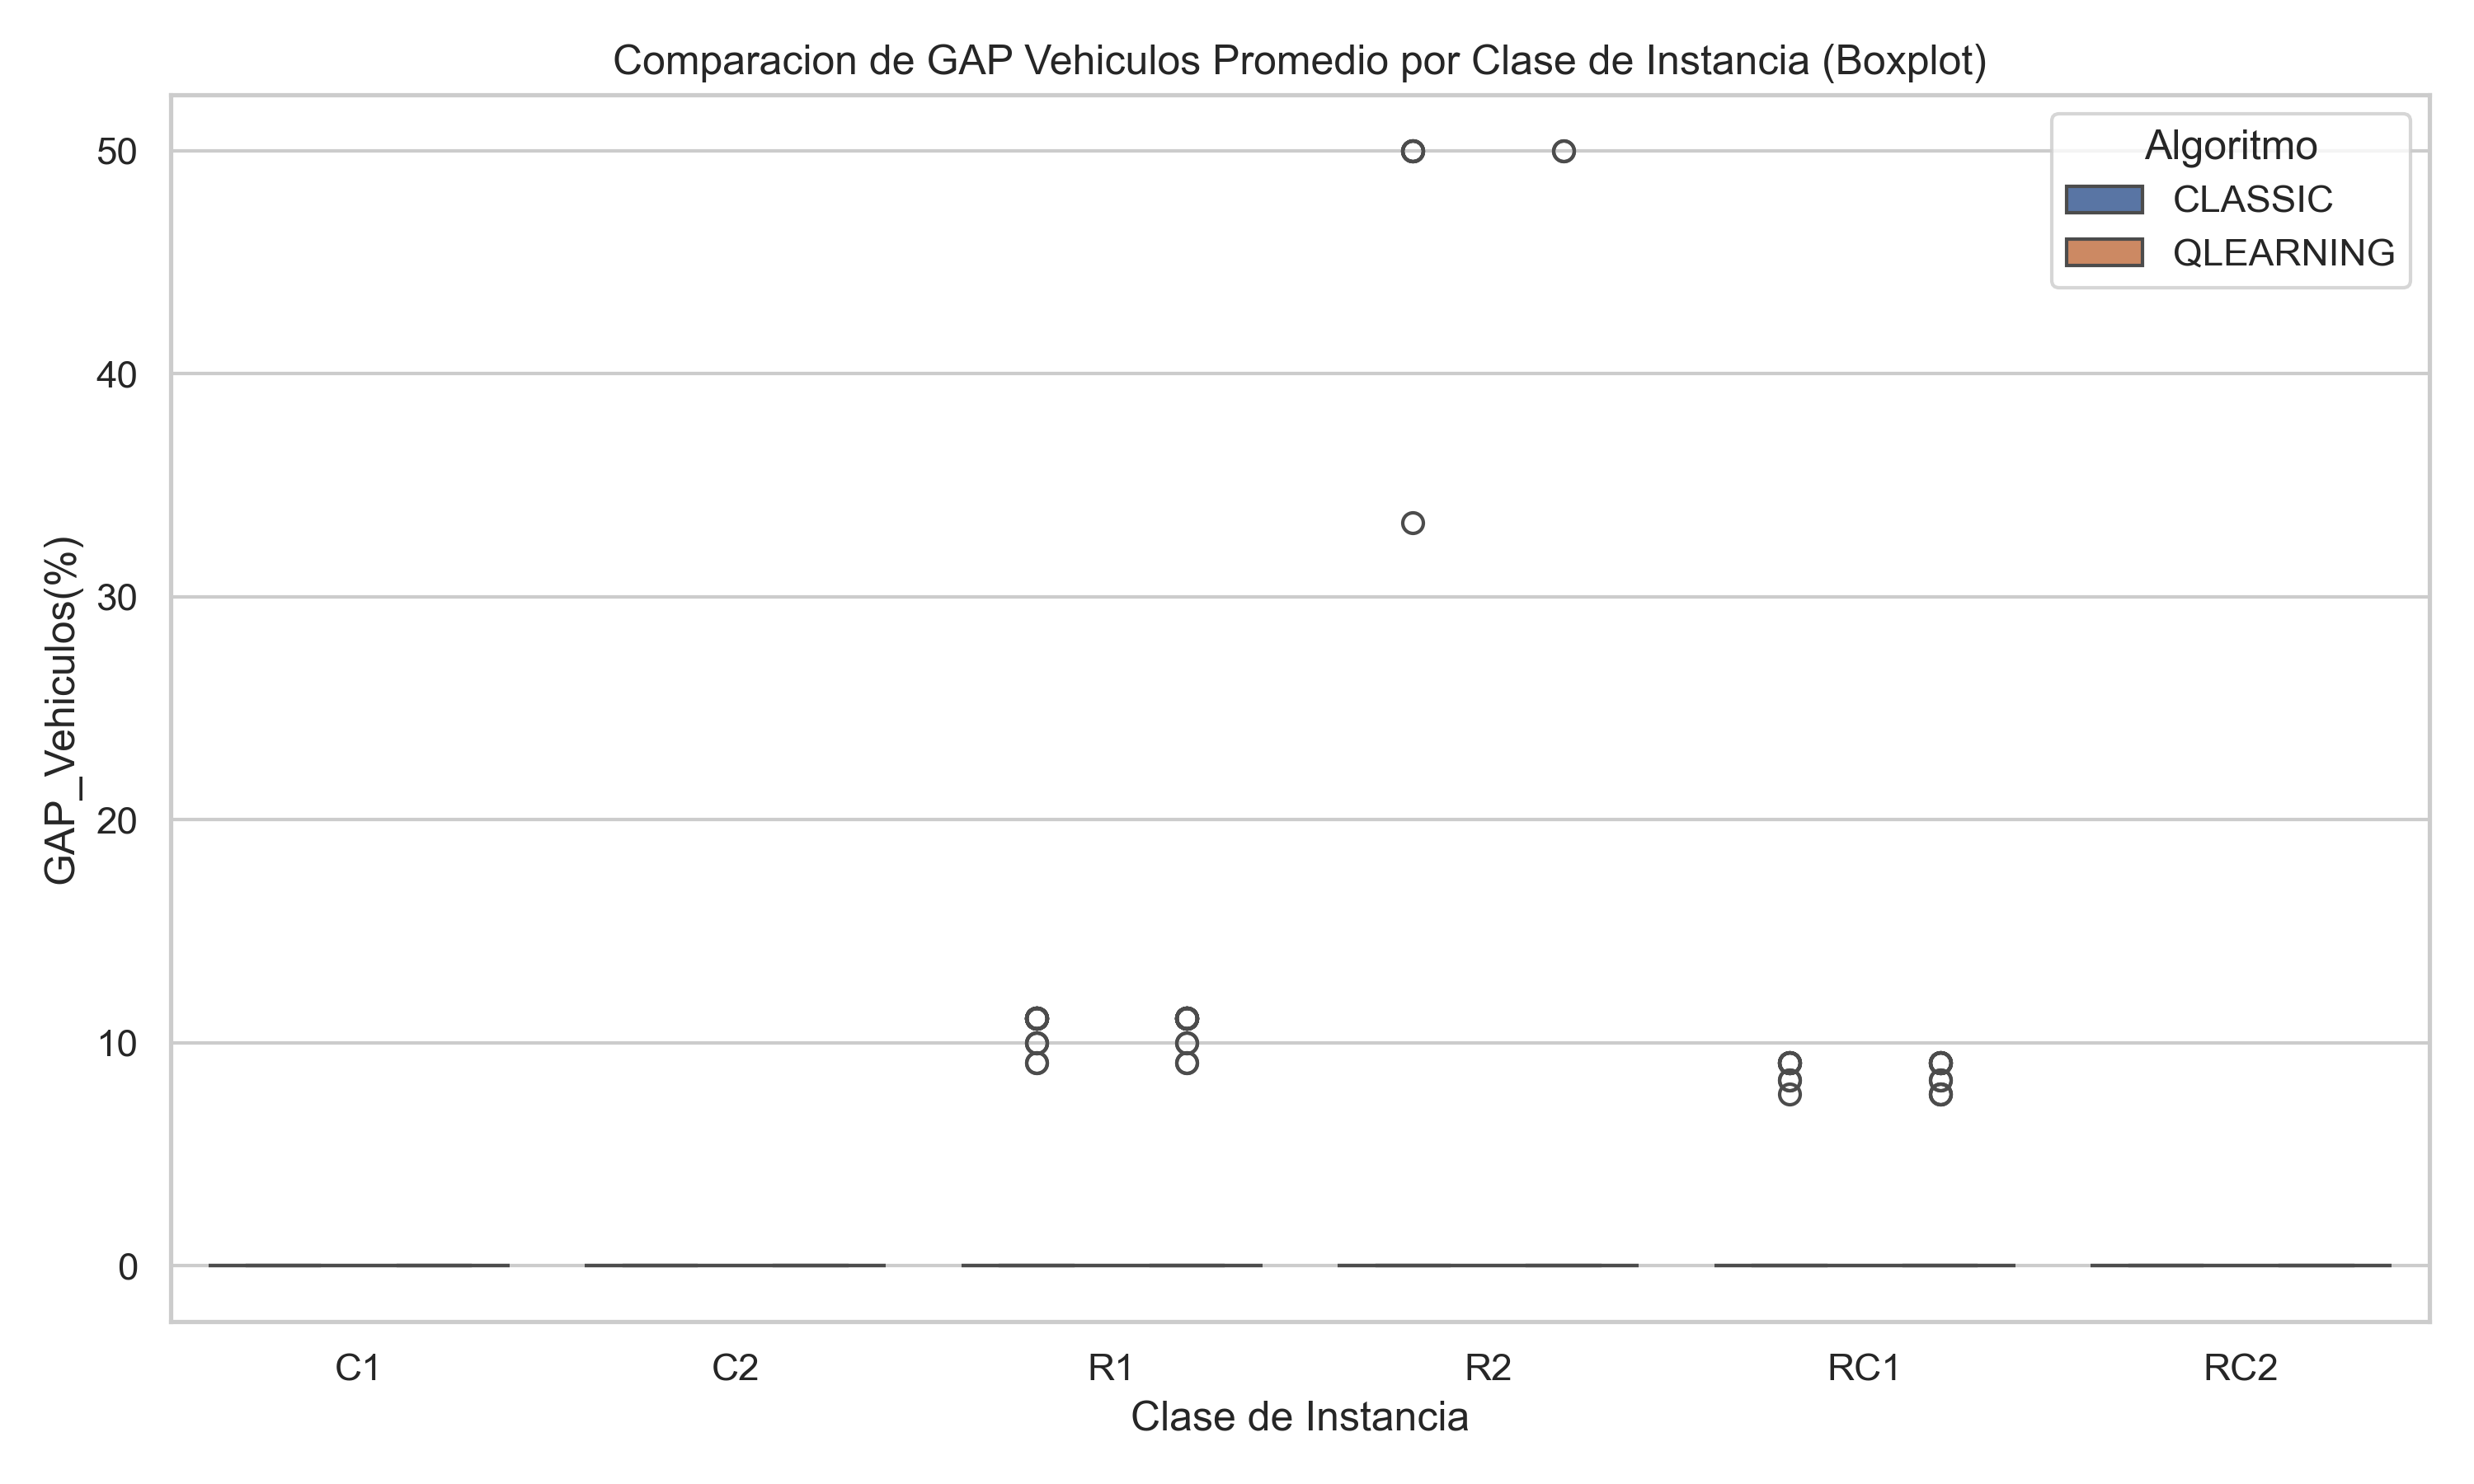
\includegraphics[width=0.78\textwidth]{../Experiments/figs/solomon/boxplot_gap_vehiculos.png}
\caption{Brecha de vehículos por corrida respecto del BKS, por clase.}
\label{fig:sol-box-veh}
\end{figure}

\begin{figure}[H]
\centering
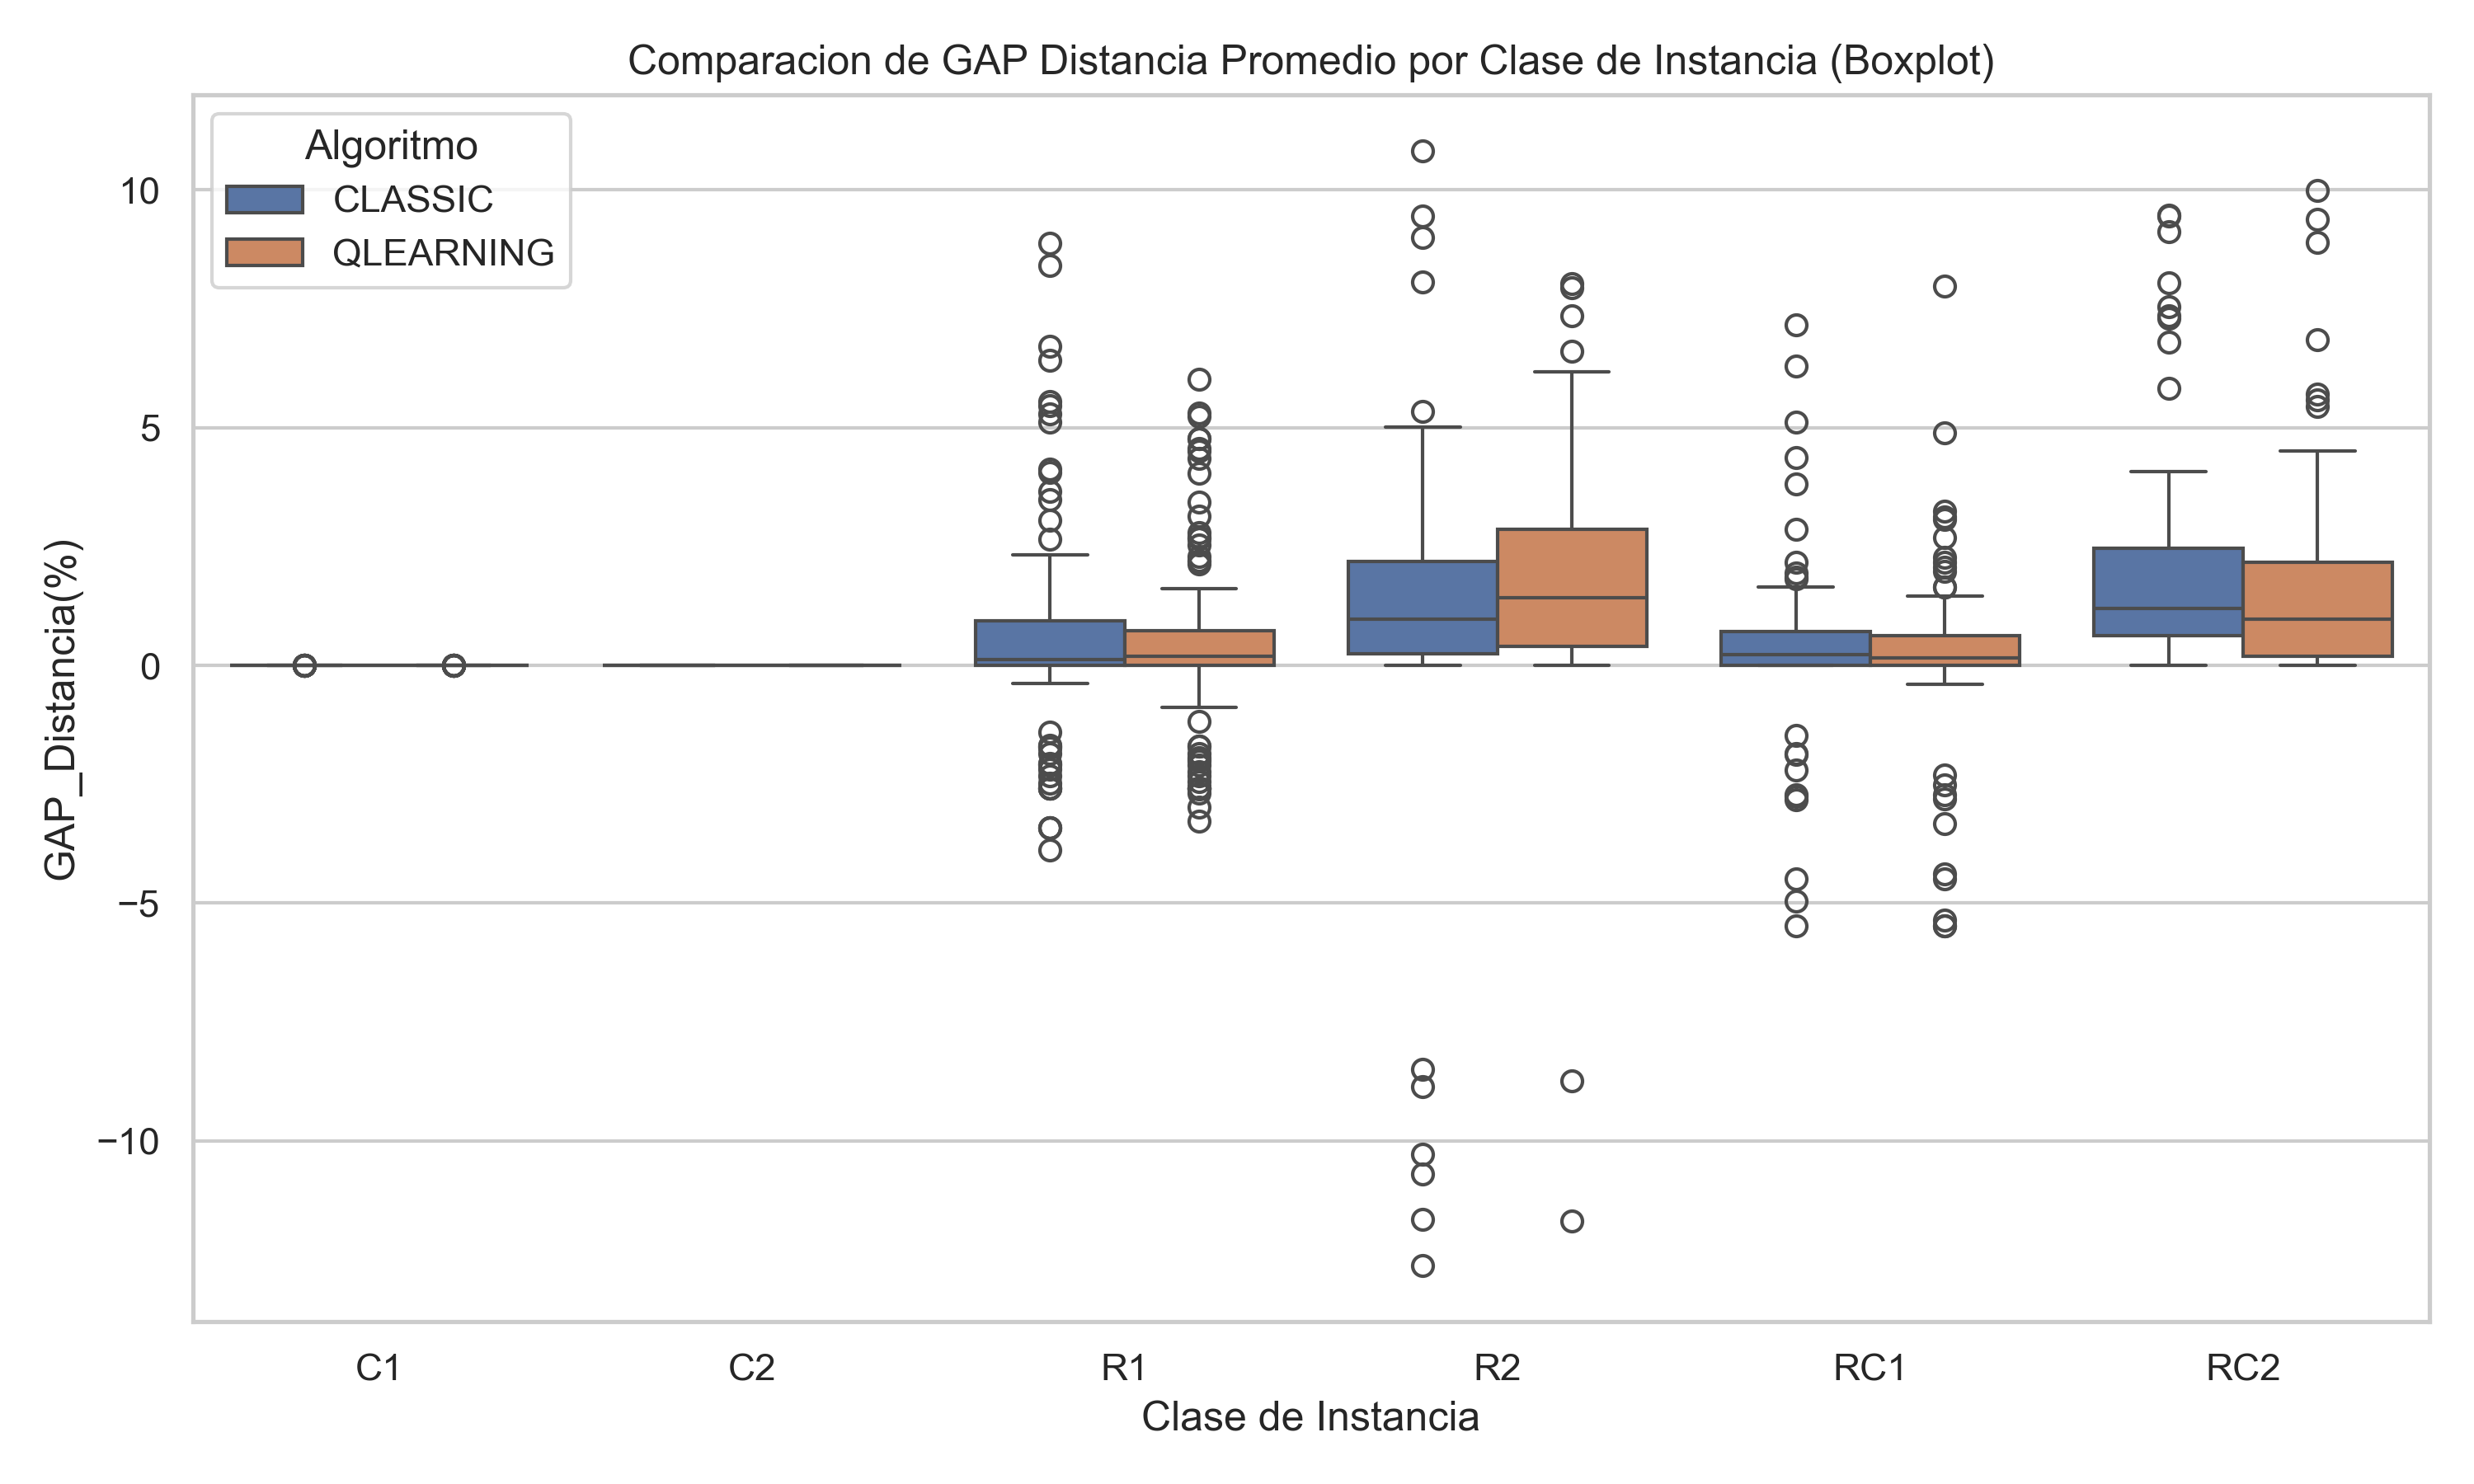
\includegraphics[width=0.78\textwidth]{../Experiments/figs/solomon/boxplot_gap_distancia.png}
\caption{Brecha de distancia por corrida respecto del BKS, por clase (sin auditar: los
valores negativos son corridas con más vehículos que el BKS).}
\label{fig:sol-box-dist}
\end{figure}

\begin{figure}[H]
\centering
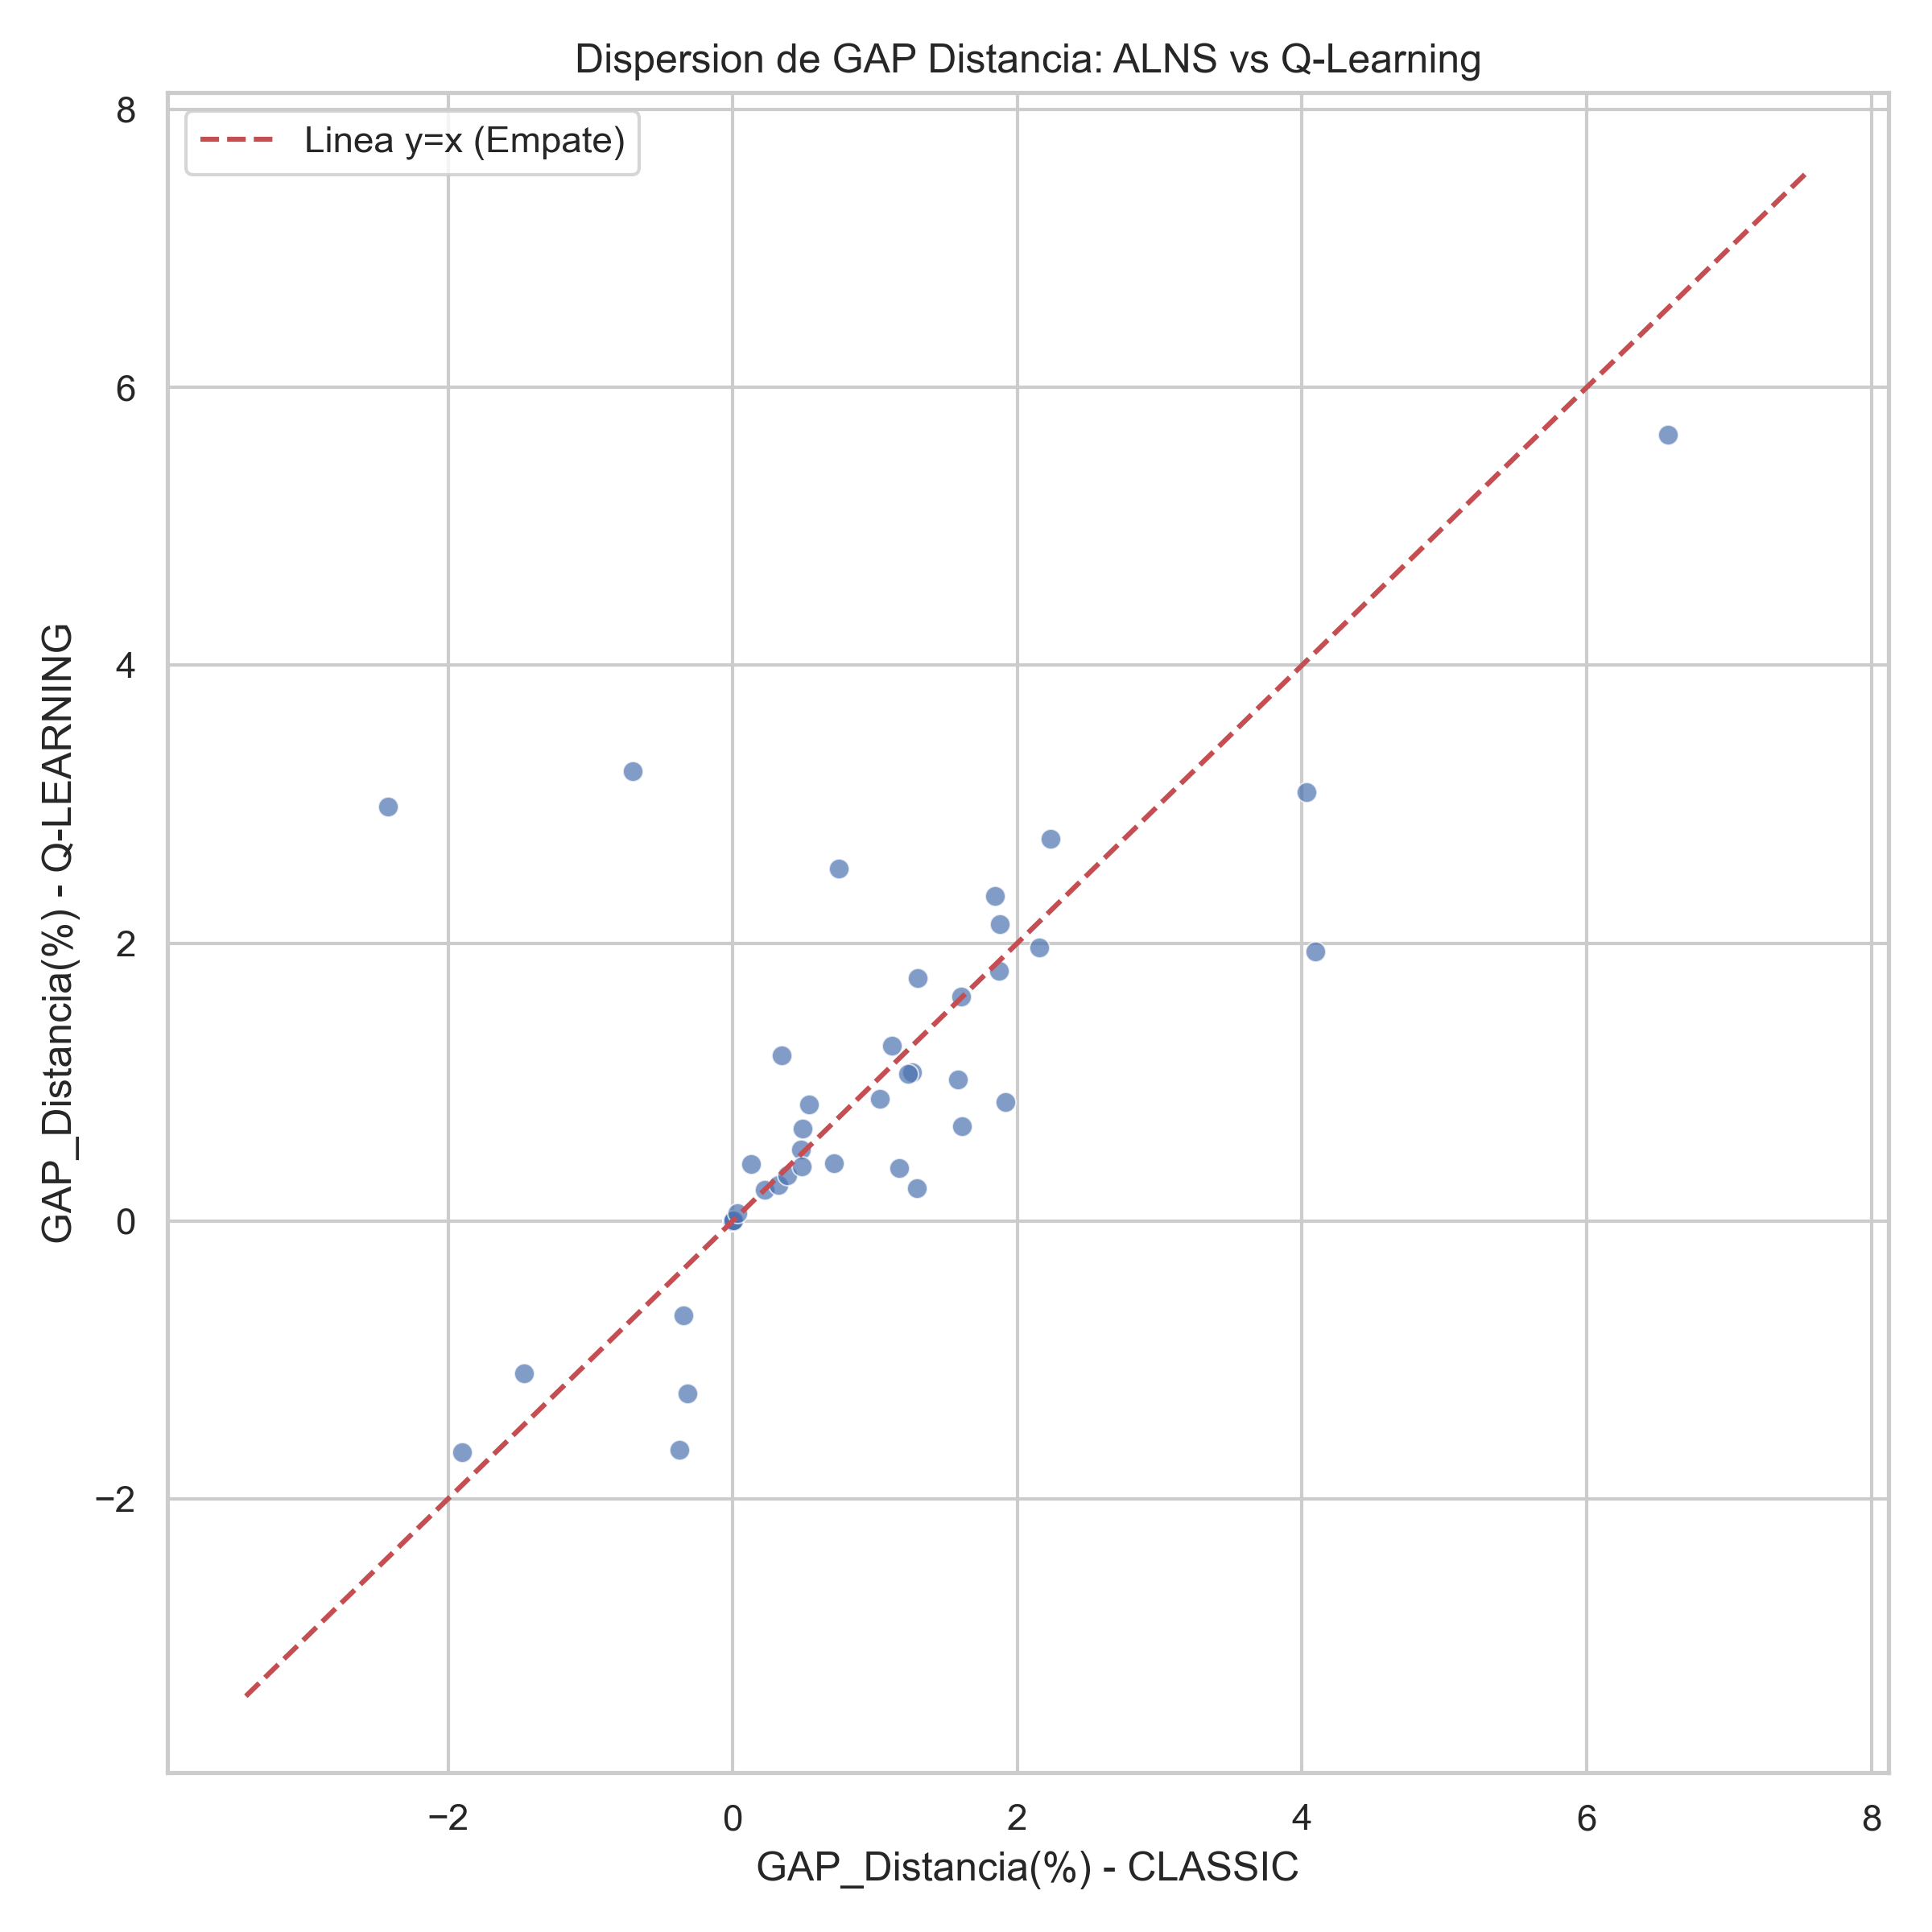
\includegraphics[width=0.6\textwidth]{../Experiments/figs/solomon/scatter_gap_distancia.png}
\caption{Brecha media de distancia por instancia: ALNS clásico (abscisas) frente a
Q-learning (ordenadas). Por debajo de la diagonal el Q-learning es mejor.}
\label{fig:sol-scatter}
\end{figure}

\subsection{Discusión}
\label{sec:exp-discusion}

\begin{itemize}
\item \textbf{Ambos métodos son competitivos en este tamaño.} Con $25\,000$ iteraciones de
fase~2 y unos $5$ segundos por corrida, los dos alcanzan la flota del BKS en todas las
instancias en al menos una de las diez corridas, y en el $93$\,\% de las corridas
individuales; la mejor corrida queda a un cuarto de punto porcentual del BKS en distancia.
Este nivel se debe a los componentes comunes (Sección~\ref{sec:sintesis}): la fase propia de
reducción de flota, el catálogo de operadores y el esquema de temperatura.
\item \textbf{No hay diferencia significativa entre los mecanismos de selección.} El
Q-learning queda ligeramente por delante en casi todos los indicadores agregados (marcador
$23$ a $16$, brecha en instancias comunes $0.70$\,\% frente a $0.79$\,\%, dos instancias más
con la flota del BKS), pero ninguna de las pruebas alcanza significación y la magnitud de las
diferencias, del orden de una décima de punto porcentual, es inferior a la variación entre
semillas. Con estos datos no puede afirmarse que un método supere al otro en instancias de
$100$ clientes.
\item \textbf{Dónde aparece la diferencia.} Las diferencias, cuando las hay, se concentran en
las clases con clientes dispersos y son nulas en las agrupadas. En R2 el Q-learning reduce
flota (iguala al BKS en $108$ de $110$ corridas, frente a $104$) a costa de distancia; en RC2,
con flota idéntica, reduce la brecha de $2.07$\,\% a $1.76$\,\%; en RC1 el clásico iguala la
flota del BKS en dos corridas más.
\item \textbf{Efecto techo.} Diecisiete de las $56$ instancias las resuelven ambos métodos en
todas las corridas, y en la mayoría de las restantes el margen respecto del BKS es inferior
al $2$\,\%. Con tan poco margen de mejora, este conjunto discrimina mal entre mecanismos de
selección: el presupuesto de iteraciones basta para que una selección menos informada llegue
a soluciones de calidad similar. Las diferencias de mecanismo descritas en la
Sección~\ref{sec:sintesis} deberían manifestarse con más claridad cuando el presupuesto es
escaso en relación con el tamaño de la instancia, lo que corresponde a las instancias de
Gehring y Homberger~\cite{gehring1999}, cuyos resultados no se incluyen en esta sección.
\end{itemize}

\subsection{Resultados por instancia}

Las Tablas~\ref{tab:sol-instancias} y~\ref{tab:sol-instancias-b} detallan las $56$ instancias. Las columnas NV y TD son medias
de las $10$ corridas; GAP es la brecha de distancia auditada, en porcentaje, y se omite (--)
cuando la flota media supera la del BKS; la mejor corrida es la mejor de las $10$ en orden
lexicográfico, expresada como vehículos/distancia.

\begin{table}[H]
\centering
\footnotesize
\setlength{\tabcolsep}{4pt}
\caption{Solomon, 100 clientes: resultados por instancia, clases C1, C2 y R1.}
\label{tab:sol-instancias}
\begin{tabular}{@{}l r r r r r r r r r r@{}}
\toprule
 & \multicolumn{2}{c}{BKS} & \multicolumn{3}{c}{ALNS clásico (media)} & \multicolumn{3}{c}{ALNS-Q (media)} & \multicolumn{2}{c}{Mejor corrida} \\
\cmidrule(lr){2-3}\cmidrule(lr){4-6}\cmidrule(lr){7-9}\cmidrule(l){10-11}
Inst. & NV & TD & NV & TD & GAP & NV & TD & GAP & ALNS & ALNS-Q \\
\midrule
% Filas generadas desde Experiments/results/solomon/master_solomon.csv
C101 & 10 & 828.94 & 10.0 & 828.94 & 0.00 & 10.0 & 828.94 & 0.00 & 10/828.94 & 10/828.94 \\
C102 & 10 & 828.94 & 10.0 & 828.94 & 0.00 & 10.0 & 828.94 & 0.00 & 10/828.94 & 10/828.94 \\
C103 & 10 & 828.06 & 10.0 & 828.07 & 0.00 & 10.0 & 828.07 & 0.00 & 10/828.07 & 10/828.07 \\
C104 & 10 & 824.78 & 10.0 & 824.78 & 0.00 & 10.0 & 824.78 & 0.00 & 10/824.78 & 10/824.78 \\
C105 & 10 & 828.94 & 10.0 & 828.94 & 0.00 & 10.0 & 828.94 & 0.00 & 10/828.94 & 10/828.94 \\
C106 & 10 & 828.94 & 10.0 & 828.94 & 0.00 & 10.0 & 828.94 & 0.00 & 10/828.94 & 10/828.94 \\
C107 & 10 & 828.94 & 10.0 & 828.94 & 0.00 & 10.0 & 828.94 & 0.00 & 10/828.94 & 10/828.94 \\
C108 & 10 & 828.94 & 10.0 & 828.94 & 0.00 & 10.0 & 828.94 & 0.00 & 10/828.94 & 10/828.94 \\
C109 & 10 & 828.94 & 10.0 & 828.94 & 0.00 & 10.0 & 828.94 & 0.00 & 10/828.94 & 10/828.94 \\
\addlinespace
C201 & 3 & 591.56 & 3.0 & 591.56 & 0.00 & 3.0 & 591.56 & 0.00 & 3/591.56 & 3/591.56 \\
C202 & 3 & 591.56 & 3.0 & 591.56 & 0.00 & 3.0 & 591.56 & 0.00 & 3/591.56 & 3/591.56 \\
C203 & 3 & 591.17 & 3.0 & 591.17 & 0.00 & 3.0 & 591.17 & 0.00 & 3/591.17 & 3/591.17 \\
C204 & 3 & 590.60 & 3.0 & 590.60 & 0.00 & 3.0 & 590.60 & 0.00 & 3/590.60 & 3/590.60 \\
C205 & 3 & 588.88 & 3.0 & 588.88 & 0.00 & 3.0 & 588.88 & 0.00 & 3/588.88 & 3/588.88 \\
C206 & 3 & 588.49 & 3.0 & 588.49 & 0.00 & 3.0 & 588.49 & 0.00 & 3/588.49 & 3/588.49 \\
C207 & 3 & 588.29 & 3.0 & 588.29 & 0.00 & 3.0 & 588.29 & 0.00 & 3/588.29 & 3/588.29 \\
C208 & 3 & 588.32 & 3.0 & 588.32 & 0.00 & 3.0 & 588.32 & 0.00 & 3/588.32 & 3/588.32 \\
\addlinespace
R101 & 19 & 1650.80 & 19.0 & 1650.85 & 0.00 & 19.0 & 1650.88 & 0.00 & 19/1650.80 & 19/1650.80 \\
R102 & 17 & 1486.12 & 17.0 & 1486.59 & 0.03 & 17.0 & 1486.95 & 0.06 & 17/1486.12 & 17/1486.12 \\
R103 & 13 & 1292.68 & 13.0 & 1295.62 & 0.23 & 13.0 & 1295.56 & 0.22 & 13/1292.68 & 13/1292.68 \\
R104 & 9 & 1007.31 & 9.9 & 988.14 & -- & 9.8 & 990.54 & -- & 9/1007.31 & 9/1007.31 \\
R105 & 14 & 1377.11 & 14.0 & 1381.53 & 0.32 & 14.0 & 1380.66 & 0.26 & 14/1377.11 & 14/1377.11 \\
R106 & 12 & 1252.03 & 12.0 & 1258.00 & 0.48 & 12.0 & 1258.45 & 0.51 & 12/1252.03 & 12/1252.03 \\
R107 & 10 & 1104.66 & 10.0 & 1118.58 & 1.26 & 10.0 & 1116.51 & 1.07 & 10/1111.44 & 10/1104.66 \\
R108 & 9 & 960.88 & 9.0 & 976.33 & 1.61 & 9.0 & 967.45 & 0.68 & 9/963.66 & 9/960.88 \\
R109 & 11 & 1194.73 & 11.2 & 1243.62 & -- & 11.2 & 1217.93 & -- & 11/1226.49 & 11/1201.41 \\
R110 & 10 & 1118.84 & 10.2 & 1127.15 & -- & 10.2 & 1147.20 & -- & 10/1118.84 & 10/1142.75 \\
R111 & 10 & 1096.73 & 10.1 & 1100.49 & -- & 10.0 & 1109.79 & 1.19 & 10/1096.73 & 10/1096.73 \\
R112 & 9 & 982.14 & 9.7 & 978.45 & -- & 9.9 & 965.98 & -- & 9/1002.26 & 9/1004.60 \\
\bottomrule
\end{tabular}
\end{table}

\begin{table}[H]
\centering
\footnotesize
\setlength{\tabcolsep}{4pt}
\caption{Solomon, 100 clientes: resultados por instancia, clases R2, RC1 y RC2.}
\label{tab:sol-instancias-b}
\begin{tabular}{@{}l r r r r r r r r r r@{}}
\toprule
 & \multicolumn{2}{c}{BKS} & \multicolumn{3}{c}{ALNS clásico (media)} & \multicolumn{3}{c}{ALNS-Q (media)} & \multicolumn{2}{c}{Mejor corrida} \\
\cmidrule(lr){2-3}\cmidrule(lr){4-6}\cmidrule(lr){7-9}\cmidrule(l){10-11}
Inst. & NV & TD & NV & TD & GAP & NV & TD & GAP & ALNS & ALNS-Q \\
\midrule
% Filas generadas desde Experiments/results/solomon/master_solomon.csv
R201 & 4 & 1252.37 & 4.0 & 1253.98 & 0.13 & 4.0 & 1257.49 & 0.41 & 4/1252.37 & 4/1253.23 \\
R202 & 3 & 1191.70 & 3.1 & 1183.33 & -- & 3.0 & 1230.30 & 3.24 & 3/1191.70 & 3/1195.30 \\
R203 & 3 & 939.50 & 3.0 & 944.52 & 0.53 & 3.0 & 947.38 & 0.84 & 3/939.50 & 3/941.41 \\
R204 & 2 & 825.52 & 2.0 & 840.99 & 1.87 & 2.0 & 843.15 & 2.14 & 2/828.78 & 2/828.78 \\
R205 & 3 & 994.43 & 3.0 & 1006.70 & 1.23 & 3.0 & 1004.94 & 1.06 & 3/994.43 & 3/994.43 \\
R206 & 3 & 906.14 & 3.0 & 920.47 & 1.58 & 3.0 & 915.34 & 1.02 & 3/906.14 & 3/906.14 \\
R207 & 2 & 890.61 & 2.1 & 926.53 & -- & 2.1 & 918.08 & -- & 2/897.06 & 2/907.69 \\
R208 & 2 & 726.82 & 2.0 & 734.33 & 1.03 & 2.0 & 733.22 & 0.88 & 2/726.82 & 2/726.82 \\
R209 & 3 & 909.16 & 3.0 & 925.92 & 1.84 & 3.0 & 930.44 & 2.34 & 3/915.24 & 3/913.77 \\
R210 & 3 & 939.37 & 3.0 & 954.42 & 1.60 & 3.0 & 954.53 & 1.61 & 3/942.11 & 3/939.37 \\
R211 & 2 & 885.71 & 2.4 & 864.27 & -- & 2.1 & 912.11 & -- & 2/901.52 & 2/900.35 \\
\addlinespace
RC101 & 14 & 1696.95 & 14.0 & 1709.01 & 0.71 & 14.0 & 1703.96 & 0.41 & 14/1697.43 & 14/1696.95 \\
RC102 & 12 & 1554.75 & 12.2 & 1549.34 & -- & 12.2 & 1544.15 & -- & 12/1554.75 & 12/1554.75 \\
RC103 & 11 & 1261.67 & 11.0 & 1267.85 & 0.49 & 11.0 & 1270.07 & 0.67 & 11/1262.02 & 11/1263.54 \\
RC104 & 10 & 1135.48 & 10.0 & 1139.86 & 0.39 & 10.0 & 1139.22 & 0.33 & 10/1135.52 & 10/1135.48 \\
RC105 & 13 & 1629.44 & 13.1 & 1624.30 & -- & 13.3 & 1609.16 & -- & 13/1629.44 & 13/1629.44 \\
RC106 & 11 & 1424.73 & 11.7 & 1403.86 & -- & 11.7 & 1409.11 & -- & 11/1424.73 & 11/1432.12 \\
RC107 & 11 & 1230.48 & 11.0 & 1246.42 & 1.30 & 11.0 & 1233.41 & 0.24 & 11/1231.53 & 11/1231.53 \\
RC108 & 10 & 1139.82 & 10.0 & 1165.29 & 2.23 & 10.0 & 1171.18 & 2.75 & 10/1146.66 & 10/1146.66 \\
\addlinespace
RC201 & 4 & 1406.94 & 4.0 & 1422.65 & 1.12 & 4.0 & 1424.72 & 1.26 & 4/1415.00 & 4/1412.45 \\
RC202 & 3 & 1365.65 & 3.0 & 1455.38 & 6.57 & 3.0 & 1442.93 & 5.66 & 3/1368.04 & 3/1365.65 \\
RC203 & 3 & 1049.62 & 3.0 & 1069.28 & 1.87 & 3.0 & 1068.53 & 1.80 & 3/1061.13 & 3/1051.82 \\
RC204 & 3 & 798.46 & 3.0 & 802.33 & 0.48 & 3.0 & 801.60 & 0.39 & 3/798.46 & 3/798.46 \\
RC205 & 4 & 1297.65 & 4.0 & 1314.51 & 1.30 & 4.0 & 1320.32 & 1.75 & 4/1303.37 & 4/1302.42 \\
RC206 & 3 & 1146.32 & 3.0 & 1168.31 & 1.92 & 3.0 & 1156.15 & 0.86 & 3/1152.03 & 3/1146.32 \\
RC207 & 3 & 1061.14 & 3.0 & 1083.97 & 2.15 & 3.0 & 1082.00 & 1.97 & 3/1070.85 & 3/1061.84 \\
RC208 & 3 & 828.14 & 3.0 & 837.82 & 1.17 & 3.0 & 831.28 & 0.38 & 3/829.70 & 3/829.70 \\
\bottomrule
\end{tabular}
\end{table}

% Referencias minimas para que el documento compile de forma autonoma.
% Al integrar en la tesis, sustituir por las entradas del gestor bibliografico
% propio (las claves \cite usadas son las de los \bibitem).
\begin{thebibliography}{9}

\bibitem{gehring1999}
H.~Gehring y J.~Homberger.
\newblock A parallel hybrid evolutionary metaheuristic for the vehicle routing problem with time windows.
\newblock En \emph{Proceedings of EUROGEN99}, pp.~57--64, 1999.

\bibitem{kirkpatrick1983}
S.~Kirkpatrick, C.~D. Gelatt y M.~P. Vecchi.
\newblock Optimization by simulated annealing.
\newblock \emph{Science}, 220(4598):671--680, 1983.

\bibitem{pisinger2007}
D.~Pisinger y S.~Ropke.
\newblock A general heuristic for vehicle routing problems.
\newblock \emph{Computers \& Operations Research}, 34(8):2403--2435, 2007.

\bibitem{ropke2006}
S.~Ropke y D.~Pisinger.
\newblock An adaptive large neighborhood search heuristic for the pickup and delivery problem with time windows.
\newblock \emph{Transportation Science}, 40(4):455--472, 2006.

\bibitem{savelsbergh1992}
M.~W.~P. Savelsbergh.
\newblock The vehicle routing problem with time windows: Minimizing route duration.
\newblock \emph{ORSA Journal on Computing}, 4(2):146--154, 1992.

\bibitem{shaw1998}
P.~Shaw.
\newblock Using constraint programming and local search methods to solve vehicle routing problems.
\newblock En \emph{Principles and Practice of Constraint Programming -- CP98}, LNCS 1520, pp.~417--431. Springer, 1998.

\bibitem{solomon1987}
M.~M. Solomon.
\newblock Algorithms for the vehicle routing and scheduling problems with time window constraints.
\newblock \emph{Operations Research}, 35(2):254--265, 1987.

\bibitem{sutton2018}
R.~S. Sutton y A.~G. Barto.
\newblock \emph{Reinforcement Learning: An Introduction}.
\newblock MIT Press, 2.\textordfeminine{} edición, 2018.

\bibitem{watkins1992}
C.~J.~C.~H. Watkins y P.~Dayan.
\newblock Q-learning.
\newblock \emph{Machine Learning}, 8(3--4):279--292, 1992.

\end{thebibliography}


\end{document}
